%----------------------------------------------------------------------------------------
%	PACKAGES AND OTHER DOCUMENT CONFIGURATIONS
%----------------------------------------------------------------------------------------

\documentclass[
11pt, % The default document font size, options: 10pt, 11pt, 12pt
%oneside, % Two side (alternating margins) for binding by default, uncomment to switch to one side
%chapterinoneline,% Have the chapter title next to the number in one single line
english, % ngerman for German
singlespacing, % Single line spacing, alternatives: onehalfspacing or doublespacing
%draft, % Uncomment to enable draft mode (no pictures, no links, overfull hboxes indicated)
%nolistspacing, % If the document is onehalfspacing or doublespacing, uncomment this to set spacing in lists to single
%liststotoc, % Uncomment to add the list of figures/tables/etc to the table of contents
%toctotoc, % Uncomment to add the main table of contents to the table of contents
%parskip, % Uncomment to add space between paragraphs
%nohyperref, % Uncomment to not load the hyperref package
headsepline, % Uncomment to get a line under the header
]{MastersDoctoralThesis} % The class file specifying the document structure

\usepackage[utf8]{inputenc} % Required for inputting international characters
\usepackage[T1]{fontenc} % Output font encoding for international characters
\usepackage{amsmath}
\usepackage{algorithmic}
\usepackage{algorithm}% http://ctan.org/pkg/algorithm
\usepackage{enumitem}
\usepackage{tikz}
\usepackage{fixltx2e}
\usepackage{graphicx}
\usepackage{longtable}
\usepackage{float}
\usepackage{wrapfig}
\usepackage{soul}
\usepackage{textcomp}
\usepackage{marvosym}
\usepackage{wasysym}
\usepackage{latexsym}
\usepackage{amssymb}
\usepackage{amsopn}
\usepackage{hyperref}
\usepackage[normalem]{ulem}
\usepackage{booktabs}
\usepackage{psfrag}
\usepackage[b]{esvect}
\usepackage{framed,color}
\setcounter{secnumdepth}{5} % seting level of numbering (default for "report" is 3). With ''-1'' you have non number also for chapters




%\setcounter{tocdepth}{5} % if you want all the levels in your table of contents
%\usepackage[noend]{algpseudocode}

\renewcommand{\algorithmicrequire}{\textbf{Input:}}
\renewcommand{\algorithmicensure}{\textbf{Output:}}


\usepackage{palatino} % Use the Palatino font by default
\usepackage{caption}
\usepackage[autostyle=true]{csquotes} % Required to generate language-dependent quotes in the bibliography



%----------------------------------------------------------------------------------------
%	MARGIN SETTINGS
%----------------------------------------------------------------------------------------

\geometry{
	paper=a4paper, % Change to letterpaper for US letter
	inner=2.54cm, % Inner margin
	outer=2.54cm, % Outer margin
	%bindingoffset=2cm, % Binding offset
	top=1.5cm, % Top margin
	bottom=1.5cm, % Bottom margin
	%showframe,% show how the type block is set on the page
}

%----------------------------------------------------------------------------------------
%	THESIS INFORMATION
%----------------------------------------------------------------------------------------

\thesistitle{Multidimensional Interpolated Discretized for Objects and Object Pairs Embedding} % Your thesis title, this is used in the title and abstract, print it elsewhere with \ttitle
\supervisor{Dr. Ofir  \textsc{Pele}} % Your supervisor's name, this is used in the title page, print it elsewhere with \supname
\examiner{} % Your examiner's name, this is not currently used anywhere in the template, print it elsewhere with \examname
\degree{Master of Science} % Your degree name, this is used in the title page and abstract, print it elsewhere with \degreename
\author{Yakir \textsc{Ben-Aliz}} % Your name, this is used in the title page and abstract, print it elsewhere with \authorname
\addresses{} % Your address, this is not currently used anywhere in the template, print it elsewhere with \addressname

\subject{Metric Learning} % Your subject area, this is not currently used anywhere in the template, print it elsewhere with \subjectname
\keywords{} % Keywords for your thesis, this is not currently used anywhere in the template, print it elsewhere with \keywordnames
\university{Ariel University of Samaria} % Your university's name and URL, this is used in the title page and abstract, print it elsewhere with \univname
\department{electrical engineering} % Your department's name and URL, this is used in the title page and abstract, print it elsewhere with \deptname
\group{Faculty of Engineering} % Your research group's name and URL, this is used in the title page, print it elsewhere with \groupname
\faculty{Faculty of Engineering} % Your faculty's name and URL, this is used in the title page and abstract, print it elsewhere with \facname

\hypersetup{pdftitle=\ttitle} % Set the PDF's title to your title
\hypersetup{pdfauthor=\authorname} % Set the PDF's author to your name
\hypersetup{pdfkeywords=\keywordnames} % Set the PDF's keywords to your keywords
\usepackage{indentfirst}
\usepackage{titlesec}

\titlespacing*{\subsection}
{0cm}{2cm}{0.3cm}
\titlespacing*{\subsection}
{1cm}{1cm}{0.3cm}

\titlespacing*{\subsubsection}
{2cm}{2cm}{0.3cm}





%----------------------------------------------------------------------------------------
%	BIBLIOGRAPHY
%----------------------------------------------------------------------------------------
\bibliographystyle{elsarticle-num}
%\bibliography{idrefs}
%% `Elsevier LaTeX' style
\usepackage[backend=bibtex,style=numeric]{biblatex}
\addbibresource{idrefs.bib}

%------------------------------------------------------------------------
\begin{document}

\frontmatter % Use roman page numbering style (i, ii, iii, iv...) for the pre-content pages

\pagestyle{plain} % Default to the plain heading style until the thesis style is called for the body content

%----------------------------------------------------------------------------------------
%	TITLE PAGE
%----------------------------------------------------------------------------------------

\begin{titlepage}
\begin{center}

{\scshape\LARGE \univname\par}\vspace{1.5cm} % University name
\textsc{\Large Masters Thesis}\\[0.5cm] % Thesis type

\HRule \\[0.4cm] % Horizontal line
{\huge \bfseries \ttitle\par}\vspace{0.4cm} % Thesis title
\HRule \\[1.5cm] % Horizontal line
 
\begin{minipage}[t]{0.4\textwidth}
\begin{flushleft} \large
\emph{Author:}\\
\href{}{\authorname} % Author name - remove the \href bracket to remove the link
\end{flushleft}
\end{minipage}
\begin{minipage}[t]{0.4\textwidth}
\begin{flushright} \large
\emph{Supervisor:} \\
\href{www.ariel.ac.il/sites/ofirpele/}{\supname} % Supervisor name - remove the \href bracket to remove the link  
\end{flushright}
\end{minipage}\\[3cm]
 
\large \textit{A thesis submitted in fulfillment of the requirements\\ for the degree of \degreename}\\[0.3cm] % University requirement text
\textit{in the}\\[0.4cm]
\groupname\\\deptname\\[2cm] % Research group name and department name
 
{\large \today}\\[4cm] % Date
%\includegraphics{Logo} % University/department logo - uncomment to place it
 
\vfill
\end{center}
\end{titlepage}

%----------------------------------------------------------------------------------------
%	DECLARATION PAGE
%----------------------------------------------------------------------------------------

%\begin{declaration}
%\addchaptertocentry{\authorshipname}
%
%\noindent I, \authorname, declare that this thesis titled, \enquote{\ttitle} and the work presented in it are my own. I confirm that:
%
%\begin{itemize} 
%\item This work was done wholly or mainly while in candidature for a research degree at this University.
%\item Where any part of this thesis has previously been submitted for a degree or any other qualification at this University or any other institution, this has been clearly stated.
%\item Where I have consulted the published work of others, this is always clearly attributed.
%\item Where I have quoted from the work of others, the source is always given. With the exception of such quotations, this thesis is entirely my own work.
%\item I have acknowledged all main sources of help.
%\item Where the thesis is based on work done by myself jointly with others, I have made clear exactly what was done by others and what I have contributed myself.\\
%\end{itemize}
% 
%\noindent Signed:\\
%\rule[0.5em]{25em}{0.5pt} % This prints a line for the signature
% 
%\noindent Date:\\
%\rule[0.5em]{25em}{0.5pt} % This prints a line to write the date
%\end{declaration}

%\cleardoublepage

%----------------------------------------------------------------------------------------
%	QUOTATION PAGE
%----------------------------------------------------------------------------------------
%
%\vspace*{0.2\textheight}
%
%\noindent\enquote{\itshape Thanks to my solid academic training, today I can write hundreds of words on virtually any topic without possessing a shred of information, which is how I got a good job in journalism.}\bigbreak
%
%\hfill Dave Barry

%----------------------------------------------------------------------------------------
%	ABSTRACT PAGE
%----------------------------------------------------------------------------------------

\begin{abstract}
\addchaptertocentry{\abstractname} % Add the abstract to the table of contents

Distance functions are at the core of numerous scientific areas. One can choose a distance function based on prior knowledge or learn it from data, metric learning. The most commonly used and learned distance function is the Euclidean distance. In metric learning, most of the works learn a Mahalanobis distance. These methods [1-12] learn a linear transform that is applied on the vector and then apply the squared Euclidean distance (thus these methods are actually semimetric learning). 
Kernel metric learning applies embedding separably on each vector before learning the linear transform. 
Deep learning methods [13] learn an embedding using a deep network and then apply the Euclidean distance on the embedded vectors (the output of the network). Thus, even kernel and deep metric learning can only learn a Euclidean distance. 
Some works [14, 15, 16, 17] have suggested learning other families of distances. However, these methods are restricted to the suggested pre-chosen families of distances (e.g. Earth Mover’s Distance and $\chi$
Finally, multi-metric learning methods [1, 18] learn separate local Mahalanobis metrics around keypoints. 
However, they do not learn a global metric. An exception is [19] which shows how to combine information from several local metrics into one global metric. 
However, again it is only able to model Euclidean metrics.

We propose a new embedding method for a single vector and for a pair
of vectors. This embedding method enables: 
\begin{itemize}[noitemsep]
	\item  efficient classification and regression of functions of single vectors
	\item  efficient approximation of distance functions
	\item  general, non-Euclidean, semimetric learning 
\end{itemize}

To the best of our prior knowledge, this is the first work that enables learning any general, non-Euclidean, semimetrics. That is, our method is a universal
semimetric learning and approximation method that can approximate any
distance function with as high accuracy and/or without semimetric
constraints.
The main difference between our model and previous models is that our model embeds object pairs jointly and not separably.
Distance between objects is the embedded vector dot product with a learned parameters vector.
Thus, most of the learning objectives are convex in our model. 
Additionally, we can enforce constraints on the vector of parameters such that the resulting distance will be a continuous semimetric. 
This work enables learning and approximation of arbitrary distance functions or arbitrary semimetrics.

\end{abstract}

%----------------------------------------------------------------------------------------
%	ACKNOWLEDGEMENTS
%----------------------------------------------------------------------------------------

\begin{acknowledgements}
\addchaptertocentry{\acknowledgementname} % Add the acknowledgements to the table of contents

The acknowledgments and the people to thank go here, don't forget to include your project advisor\ldots

\end{acknowledgements}

%----------------------------------------------------------------------------------------
%	LIST OF CONTENTS/FIGURES/TABLES PAGES
%----------------------------------------------------------------------------------------

\tableofcontents % Prints the main table of contents

\listoffigures % Prints the list of figures

\listoftables % Prints the list of tables

\listofalgorithms

%----------------------------------------------------------------------------------------
%	ABBREVIATIONS
%----------------------------------------------------------------------------------------

\begin{abbreviations}{ll} % Include a list of abbreviations (a table of two columns)

\textbf{ID} & Interpolized Discretized \\
\textbf{NDIDD} & n-Dimension Interpolized Discretized Distance \\
\textbf{BCC} & Bary centric coordinates \\ 
\textbf{SGD} & Stochastic Gradient Descent

\end{abbreviations}

%----------------------------------------------------------------------------------------
%	PHYSICAL CONSTANTS/OTHER DEFINITIONS
%----------------------------------------------------------------------------------------

%\begin{constants}{lr@{${}={}$}l} % The list of physical constants is a three column table

% The \SI{}{} command is provided by the siunitx package, see its documentation for instructions on how to use it

%	Speed of Light & $c_{0}$ & \SI{2.99792458e8}{\meter\per\second} (exact)\\
%Constant Name & $Symbol$ & $Constant Value$ with units\\

%\end{constants}

%----------------------------------------------------------------------------------------
%	SYMBOLS
%----------------------------------------------------------------------------------------
%
%\begin{symbols}{lll} % Include a list of Symbols (a three column table)
%
%$a$ & distance & \si{\meter} \\
%$P$ & power & \si{\watt} (\si{\joule\per\second}) \\
%Symbol & Name & Unit \\
%
%\addlinespace % Gap to separate the Roman symbols from the Greek
%
%$\omega$ & angular frequency & \si{\radian} \\
%
%\end{symbols}

%----------------------------------------------------------------------------------------
%	DEDICATION
%----------------------------------------------------------------------------------------

\dedicatory{/Dedicated to/To my\ldots} 




%----------------------------------------------------------------------------------------
%	THESIS CONTENT - CHAPTERS
%----------------------------------------------------------------------------------------

\mainmatter % Begin numeric (1,2,3...) page numbering

\pagestyle{thesis} % Return the page headers back to the "thesis" style

% Include the chapters of the thesis as separate files from the Chapters folder
% Uncomment the lines as you write the chapters

% Chapter 1

\chapter{Introduction} % Main chapter title

\label{Chapter1} % For referencing the chapter elsewhere, use \ref{Chapter1} 

%----------------------------------------------------------------------------------------

% Define some commands to keep the formatting separated from the content 
\newcommand{\keyword}[1]{\textbf{#1}}
\newcommand{\tabhead}[1]{\textbf{#1}}
\newcommand{\code}[1]{\texttt{#1}}
\newcommand{\file}[1]{\texttt{\bfseries#1}}
\newcommand{\option}[1]{\texttt{\itshape#1}}

%----------------------------------------------------------------------------------------

%\section{Welcome and Thank You}
Distance functions are at the core of numerous scientific areas , such as classification, regression, clustering challenges etc.
it can be based either on strict, constant formulation, such as norms \cite{trefethen1997numerical} (such as $L_2$ norm, representing the euclidean distance \cite{danielsson1980euclidean}), or can be learned from datasets - metric learning.

In metric learning, most of the works learn a Mahalanobis distance \cite{de2000mahalanobis}. These methods learn a linear transformation that is applied on the vector and then apply the squared Euclidean distance (thus these methods are actually semimetric learning). 
Kernel metric learning applies embedding separably on each vector before learning the linear transformation. 
Deep learning \cite{lecun2015deep} methods learn an embedding using a deep network and then apply the Euclidean distance on the embedded vectors (the output of the network). Thus, even kernel and deep metric learning can only learn a Euclidean distance. 
Some works [14, 15, 16, 17] have suggested learning other families of distances. However, these methods are restricted to the suggested pre-chosen families of distances (e.g. Earth Mover’s Distance and $\chi$.
Finally, multi-metric learning methods [1, 18] learn separate local Mahalanobis metrics around
keypoints. However, they do not learn a global metric. An exception is [19] which shows how
to combine information from several local metrics into one global metric. However, again it is only able to model Euclidean metrics.

\vskip30pt
Our work is handling the following use case: let us say there is a given dataset, which does not own any euclidean properties, and cannot be embedded separately in order to perform various classification tasks. 
Ofir’s work \cite{ofirpelethesis} treats this particular matter, by interpolating and embedding pairs of data as a unified objects, by performing bin to bin semi-metric pairing.

We propose a new embedding method for a single vector and for a pair
of vectors. This embedding method enables: 
\begin{itemize}[noitemsep]
	\item  efficient classification and regression of functions of single vectors
	\item  efficient approximation of distance functions
	\item  general, non-Euclidean, semimetric learning 
\end{itemize}

Bin to bin comparison between pairs of data samples is beneficial when the data is not dimensionally correlated, and has no relations between one dimension in the first vector, to another. For example, when performing SIFT \cite{brown2007automatic} analysis to compare between two images for pattern recognition, there might be relations between one element to its own neighbors, but also to its paired - candidate neighbor.
For this and other purposes we may consider a cross-bin comparison method.

Let us now address describing the theories behind our method.

%----------------------------------------------------------------------------------------

\section{Metrics}


\subsection{Definition}

\textbf{Metric space} is a set for which distances between all members of the set are defined. Distances applied on every pair of objects on a given set called \textbf{metric}.
A metric $d$ is defined as:\\
\begin{equation}
d: q_1 \times q_2 \rightarrow \Re
\end{equation}
where $q_i$ are objects in a given set

\subsection{Metrics Properties}
Any metrics must obey the following properties:

\subsubsection{Non-negativity}  \label{sec:1}
any metric on a pair of objects must be non-negative
\begin{equation}
d(q_1,q_2) \geq 0
\end{equation}

\subsubsection{Identity of Indiscernibles}  \label{sec:2}
\begin{equation}
d(q_1,q_2) = 0 \iff q_1 = q_2
\end{equation}
for every pair of objects $q_1,q_2$, $d$ metric function provides zero if and only if those objects are identical.
Identity of indiscernibles is an ontological principle that states there cannot be separate objects or entities that have all their properties in common.


\subsubsection{Symmetry} \label{sec:3}
\begin{equation}
d(q_1,q_2) = d(q_2,q_1)
\end{equation}
A symmetric function of a pair of objects is one whose value at any pair of objects is the same as its value at any permutation of that pair. 

\subsubsection{Sub-additivity (Triangle Inequality)} \label{sec:4}
\begin{equation}
d(q_1,q_3) \leq d(q_1,q_2) + d(q_2,q_3)
\end{equation}
Evaluating the function for the sum of two elements of the domain always returns something less than or equal to the sum of the function's values at each element. 
\\
There are two useful generalizations for metric definition:

\subsection{Semi-metrics}
Semi metric is a generalization of the metric definition, which basically excludes \ref{sec:4}, and remains the rest.
\subsection{Pseudo-metrics}
Pseudometrics supports all metrics properties except the identity of indiscernibles property \ref{sec:2}, which is modified as follows:
\begin{equation}
q_1 = q_2 \Rightarrow d(q_1,q_2) = 0
\end{equation}


\section{Metric Learning}

Metric learning study refers to learning a distance function from data objects, while still applying the basic properties of metrics.

Most of the works learn a Mahalanobis distance[]. These methods [1-12] learn a linear transform that is applied on the vector and then apply the squared Euclidean distance (thus these methods are actually semimetric learning). 
\\\textbf{Kernel metric learning} applies embedding separably on each vector before learning the linear transform. 
\\\textbf{Deep learning} methods such [13] learn an embedding using a deep network and then apply the Euclidean (or any known) distance on the embedded vectors (the output of the network). 
Thus, even kernel and deep metric learning can only learn a Euclidean distance. Some works [14-17] have suggested learning other families of distances. 
However, these methods are restricted to the suggested pre-chosen families of distances (e.g. Earth Mover’s Distance[] and $\chi^2$[].\\
Finally, multi-metric learning methods [1, 18] learn separate local Mahalanobis metrics around keypoints. However, they do not learn a global metric. An exception is [19] which shows how to combine information from several local metrics into one global metric. However, again it is only able to model Euclidean metrics.




\section{Bin-to-Bin \& Cross-Bin Metrics}
Bin-to-Bin distance functions such as $L_2, L_1$ and $\chi^2$ compare only corresponding bin’s of a vector to its exact corresponding bin in the second vector. The assumption when using these distances is that the histogram domains are aligned. However this assumption is violated in many cases due to quantization, shape deformation, light changes, etc. Bin-to-bin distances depend on the number of bins. If it is low, the distance is robust, but not discriminative, if it is high, the distance is discriminative, but not robust. 
Distances that take into account cross-bin relationships (cross-bin distances) can be both robust and discriminative.


\section{Mahalanobis Distance}
Let $A \in \Re^{N \times N}$ be a bin-similarity matrix, so that $a_ij$ encodes how much bin i is similar to bin j. \\
The Quadratic-Form (QF) distance [21] is defined as : 
\begin{equation}
QF^A(P, Q) = \sqrt{(P - Q)^T \times A(P - Q)}
\end{equation}
Where the bin-similarity matrix $A$ is the inverse of the covariance matrix, the $QF$ distance is called the Mahalanobis distance [22]. If the bin-similarity matrix is positive-semidefinitive (PSD), $A$ matrix can be expressed as $A = LL^T$ for some real matrix $L$. Thus, the distance can be computed as the Euclidean norm between linearly transformed vectors: 
\begin{equation}
QF^A(P, Q) = \lVert LP - LQ \rVert_2
\end{equation}


In this case the QF distance is a \textbf{psuedo-metric}


\section{Related Work}

Our method builds in a novel direction on the success of previous metric learning approaches. As Weinberger and Saul \cite{weinberger2009distance} conjectured, more adaptive transformations of the input space can lead to improved performance. Our method allows to enlarge the number of the learned parameters, while the computation of the distance between two never-seen examples is only linear in the dimension. 

Chopra et al. \cite{chopra2005learning} proposed to learn a convolutional neural net as a nonlinear transformation before applying the ℓ2 norm. They showed excellent results on image data. 
Babenko et al. [] suggested a boosting framework for learning non-Mahalanobis metrics. They also presented excellent results on image data. These methods are non-convex and thus they might suffer from local minimas and training is sensitive to parameters. 

Kernel methods were also proposed in order to learn a Mahalanobis distance over non-linear transformations of the data [1, 7, 9]. Computing such a distance between two vectors scales linear in the number of training examples, which makes it impractical for large datasets. Computing our ID distances does not depend on the number of training examples. 

A family of non-Mahalanobis distances recently proposed is the Quadratic-Chi (QC) [15]. The QC family generalizes both the Mahalanobis distance and the χ 2 distance. A QC distance have parameters that can be learned. However, a serious limitation is that it can only model χ 2 -like distances. In addition, it is applicable only to non-negative vectors. Finally, it is non-convex with respect to its parameters, so learning them is hard. 

Rosales and Fung [5] also propose learning metrics via linear programming. However, while we learn a non-Mahalanobis distance, their method learns a subfamily of Mahalanobis distance. That is, their method is restricted to learning a Mahalanobis distance which is parameterized with a diagonal dominant matrix. 

Danfeng et al. [3]  displays a Quantized Kernels metrics learning methods concludes additive and block-wise kernels learning. Our method refers to any multi-dimensional distance learning problem, not only blocks of objects (such as SIFT descriptor maps around any interest point of an image)


\section{Contribution}

In this novel work, we present an efficient method for embedding either single object or pairs of objects.
This method applies a semi-metric learning for a given data space. This method is a generalization of the single-dimensional Interpolated-Discretized (ID) distance, presented by Dr. Ofir Pele \cite{ofirpelethesis}. 
In this work we embed pairs of objects jointly, which for our best of knowledge is the debut embedding method for such purpose.
In this work a novel attitude for upgrading IDD embedding procedure to n-dimensional IDD, while maintaining its basic semi-metric, non-euclidean properties, and also contributes the ability of applying “physical” constraints during the embedding process to maintain our method continuous and linearly computed. 


% Chapter 1

\chapter{ID Embedding} % Main chapter title

\label{Chapter2} % For referencing the chapter elsewhere, use \ref{Chapter1} 

%----------------------------------------------------------------------------------------

% Define some commands to keep the formatting separated from the content 
%\newcommand{\keyword}[1]{\textbf{#1}}
%\newcommand{\tabhead}[1]{\textbf{#1}}
%\newcommand{\code}[1]{\texttt{#1}}
%\newcommand{\file}[1]{\texttt{\bfseries#1}}
%\newcommand{\option}[1]{\texttt{\itshape#1}}

%----------------------------------------------------------------------------------------

We now describe the general embedding process for both single objects and object pairs. This is the core process applied on several tasks in our work, such classification, regression, pairs matching etc.
Our embedding method is assembled from three main phases:

\begin{itemize}
	\item Discretization
	\item Interpolation
	\item Assigning
\end{itemize}

let us describe each part in the ID sequence:

\section{Discretization}
Discretization phase is performed in order to downgrade complexity of a given machine/metric learning problem. 
Let us assume we have a very high ordered vectors to classify, for example a 1G ordered vectors dataset $\overrightarrow{v} \in \Re^{10^9}$ would cause struggled learning process due to high memory resources required.

For that reason we downscale problems’ dimensions by discretizing the dataset in the following \textbf{dimension-wise} method:
Each dimension in dataset is clustered and sorted into $C_i$ - dimensional $\overrightarrow{v} \in \Re^{C_i}$ vector.\\
Any common clustering method may benefit in this, with one exception:
The extremum points of the sorted discretized vector must surround the extremum values of the dataset.

\section{Interpolation}

As described above, our IDD function should delivers continuous output for any given valid object/pair of objects. 
For this purpose we perform interpolation of the given data sample features, where each element among data sample is interpolated by its closest boundaries in the proper discretization vector space. By the following algorithm:

\begin{enumerate}
	\item For each element find closest bounds among discretization vector
	\item Compute coefficients - this will be described further for every scenario, where this phase is actually performs a multidimensional interpolation
	
\end{enumerate}
\section{Assigning}

This phase assigns the coefficients computed in the last phase, in their proper locations among the embedded (sparsed) vector.

In the following sections we describe specifically each nuance of each sub-domain of the method. Please notice that the most detailed sub-method in this work is the multidimensional IDD pairs embedding, since it is the most innovative section in this work in our opinion.

		\begin{algorithm}
			\caption{Embedding Method - General}
			\begin{algorithmic}
			 
			
			\REQUIRE $L$ sized, vectorized n-dimensional dataset
			\REQUIRE number of centers per dimension - $C$
			\ENSURE $\overrightarrow{\phi}$: $L$ sized set, embedded, sparse vectors\\
			
			\STATE Find centers vectors
			\STATE V shall be a set of centers vectors
			\FORALL{dim in $n$}  
			\STATE $V_{dim} \leftarrow centers \quad vector \quad per \quad dim$
			\ENDFOR
			
			\STATE Find embedded coefficients for all dataset
			\STATE $\overrightarrow{\phi} = C^n$ length empty $\overrightarrow{\phi}$ embedded vectors
			\FORALL{$vec$ in $L$}
			\STATE find $vec$ bounding hypercube 
			\STATE find $vec$ bounding simplex (permutation method)
			\STATE $\overrightarrow{\lambda} \leftarrow$ find $vec$ barycentric coefficients 
			\STATE $\overrightarrow{\hat{\lambda}} \leftarrow$ normalize($\overrightarrow{\lambda}$)
			\ENDFOR
			\STATE Assign
			\FORALL{$\overrightarrow{evec}$ in $emb-set$}
			\STATE $inds \leftarrow$ find vertices from hypercube and simplex locations
			\FORALL{$i$ in $inds$}
			\STATE $\overrightarrow{evec}(i) \leftarrow \overrightarrow{\hat{\lambda}}(j(i))$ -- j is the assigning function between the coef. vector and embedding vector
			\ENDFOR
			\ENDFOR
			
			\RETURN $\overrightarrow{\phi}$

			
			\end{algorithmic}
		\end{algorithm}
	 
	



\chapter{Interpolated Discretized object pairs embedding} % Main chapter title

\label{Chapter3} % For referencing the chapter elsewhere, use \ref{Chapter1} 

We now describe the Interpolated Discretized Distances (IDD) embedding method.
As mentioned above, this method uniqueness is applying an embedding method that treats each pair as a \textbf{joint} object in its problem.
This method may fit any two-objects task such similarity/matching problems etc. 
Let us initiate by presenting the original single dimensional (IDD-1D) work \cite{ofirpelethesis}, then the expansion of this work into multidimensional (IDD-ND) scenario - general distance embedding is described.

\section{1D case}

	Our method's objective is to find an embedding function such:
	\begin{equation}
		ID:\Re^n \times \Re^m \rightarrow \Re^d
	\end{equation}
	, which applies the following distance function by multiplying with a learned weights vector $\overrightarrow{w}$ (learned vector)
	
	\begin{equation}
	d(\overrightarrow{x_1} , \overrightarrow{x_2}) = ID(\overrightarrow{x_1} , \overrightarrow{x_2}) \times \overrightarrow{w}
	\end{equation}
	
	this embedding shall obtain semimetric constraints applied.
	
	\subsection{Discretization}

%	\begin{}

	$	\qquad \qquad \qquad \quad \begin{pmatrix} c_{1(1)} , \dots , \dots , \dots , c_{1(n)} \end{pmatrix}\\
		
		W =		\begin{pmatrix} c_{2(1)} \\ \vdots \\ \vdots \\ \vdots \\ \vdots \\c_{2(m)} \end{pmatrix}
		\begin{pmatrix}
			s_{1,1}&   \dots&   \dots&   \dots& s_{1,m}\\
			\vdots& \ddots &        &        & \vdots \\
			\vdots&        & \ddots &        & \vdots  \\
			\vdots&        &        & \ddots & \vdots  \\
			\vdots&        &        &        & \vdots  \\
			s_{n,1}  & \dots  & \dots  & \dots  & s_{n,m}
		\end{pmatrix} $ \\ 
		\caption[discretization matrix]
		{discretization matrix $W$ as built from 2 vectors $c_1 , c_2$. this matrix is 2D as it is an outcome of 2 - 1D vectors discretization processes}
	\end{figure}

	
	as described in \ref{Chapter2}, $1D-IDD$ describes bin-to-bin distance between two samples from single dimensional spaces. Each dimension is clustered and sorted into $C_i$ - dimensional: $\overrightarrow{c} \in \Re^{C_i}$ vector.
	The vector's pair defines the shape of a distance matrix $W \in \Re^{C_i \times C_j}$ , where each element $W_i,j$ describes the distance between two cluster centers form vectors - $v_a , v_b$ \\
	
	
	
	\subsection{Interpolation}
	
	As described above , our $IDD$ function provides continuous output for any given valid object/pair of objects. 
	For this purpose we perform interpolation of the given data sample features within the $W$ matrix space for each data sample by the following process:
	\begin{itemize}
		\item extract the closest vertices from $W$ matrix to the feature sample. 
		\item calculate four (2 per feature) coefficients per sample, each represented by the normalized surface of the opposite triangle to a vertex (1D coefficients calculation will be described in section). 
		\item 1D-IDD is computed by applying inner product between the sparse coefficient vector and their corresponding vertices vector:\\
		\begin{equation}
		1DIDD = \sum_{t=1}^{3}\alpha_{a(t),b(t)} \times W_{a(t),b(t)}
		\end{equation}
		where:\\
		$\alpha$ is the coefficients sparse vector , representing the interpolation result per feature vector
		$a , b$ are parametrization function for both $\alpha , W$
		$t$ is the scanning index for all arguments among this expression
	\end{itemize}
	
	\begin{figure}
	  \centering
	  	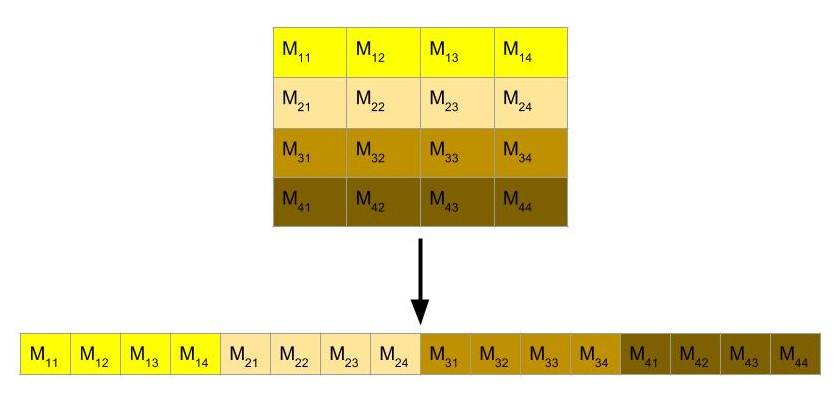
\includegraphics[width=\linewidth,height=12cm,keepaspectratio]{Figures/flatten}

	  \caption{Close-up of a gull}
	  \label{fig:gull}
	\end{figure}
	Figure \ref{fig:gull} shows a photograph of a gull.	
	Please notice that there are only 4 elements different than zero at $\alpha$, so this expression represents the non-zero elements only provides value to $1DIDD$ expression \\
	
	$a,b$ parameterizations are described as:
	
	\begin{itemize} \label{hypercubes}
		\item	\begin{equation} a_{(1)}=a{(2)} =argmax_{(c_i)} \{ v_{c_i} \leq x_i \} \end{equation}
		\item 	\begin{equation} a_{(3)}=a{(4)} =argmin_{(c_i)} \{ v_{c_i} \geq x_i \}  \end{equation} 
		\item 	\begin{equation} b_{(1)}= b_{(3)} =argmax_{(c_j)} \{ v_{c_j} \leq x_j \}  \end{equation}
		\item 	\begin{equation} b_{(2)}=b_{(4)} =argmin_{(c_j)} \{ v_{c_j} \geq x_j \} \end{equation} 
	\end{itemize}		
	
	\subsubsection{Interpolation Coefficients extraction - 1D}
	
	Let us describe how does coefficients vectors are calculated from a data sample (assembled from a pair of samples) and a discretization matrix.
		
		
	\newcommand{\MyNewVariable}{(0.3 , 0.8)}
				
	\begin{figure}[h]
			\centering
			\scalebox{0.6}
			{
				\begin{tikzpicture}[scale=5]
				\tikzstyle{vertex}=[circle,minimum size=20pt,inner sep=0pt]
				\tikzstyle{selected vertex} = [vertex, fill=red!6]
				\tikzstyle{selected edge} = [draw,line width=5pt,-,blue!50]
				\tikzstyle{edge} = [draw,thick,-,black]

				
				%\node[vertex] (v00) at (-3,-3) {$(-3,-3)$};
				\node[vertex] (v01) at (-3,-2) {$(-3,-2)$};
				\node[vertex] (v02) at (-3,-1) {$(-3,-1)$};
				\node[vertex] (v03) at (-3,0) {$(-3,0)$};
				\node[vertex] (v04) at (-3,1) {$(-3,1)$};
				\node[vertex] (v05) at (-3,2) {$(-3,2)$};
				\node[vertex] (v06) at (-3,3) {$(-3,3)$};
				%\node[vertex] (v10) at (-2,-3) {$(-2,-3)$};
				\node[vertex] (v11) at (-2,-2) {$(-2,-2)$};
				\node[vertex] (v12) at (-2,-1) {$(-2,-1)$};
				\node[vertex] (v13) at (-2,0) {$(-2,0)$};
				\node[vertex] (v14) at (-2,1) {$(-2,1)$};
				\node[vertex] (v15) at (-2,2) {$(-2,2)$};
				\node[vertex] (v16) at (-2,3) {$(-2,3)$};
				%\node[vertex] (v20) at (-1,-3) {$(-1,-3)$};
				\node[vertex] (v21) at (-1,-2) {$(-1,-2)$};
				\node[vertex] (v22) at (-1,-1) {$(-1,-1)$};
				\node[vertex] (v23) at (-1,0) {$(-1,0)$};
				\node[vertex] (v24) at (-1,1) {$(-1,1)$};
				\node[vertex] (v25) at (-1,2) {$(-1,2)$};
				\node[vertex] (v26) at (-1,3) {$(-1,3)$};
				%\node[vertex] (v30) at (0,-3) {$(0,-3)$};
				\node[vertex] (v31) at (0,-2) {$(0,-2)$};
				\node[vertex] (v32) at (0,-1) {$(0,-1)$};
				\node[vertex] (v33) at (0,0) {\textcolor{green}{$(0,0)$}};
				\node[vertex] (v34) at (0,1) {\textcolor{red}{$(0,1)$}};
				\node[vertex] (v35) at (0,2) {$(0,2)$};
				\node[vertex] (v36) at (0,3) {$(0,3)$};
				%\node[vertex] (v40) at (1,-3) {$(1,-3)$};
				\node[vertex] (v41) at (1,-2) {$(1,-2)$};
				\node[vertex] (v42) at (1,-1) {$(1,-1)$};
				\node[vertex] (v43) at (1,0) {$(1,0)$};
				\node[vertex] (v44) at (1,1) {\textcolor{blue}{$(1,1)$}};
				\node[vertex] (v45) at (1,2) {$(1,2)$};
				\node[vertex] (v46) at (1,3) {$(1,3)$};
				%\node[vertex] (v50) at (2,-3) {$(2,-3)$};
				\node[vertex] (v51) at (2,-2) {$(2,-2)$};
				\node[vertex] (v52) at (2,-1) {$(2,-1)$};
				\node[vertex] (v53) at (2,0) {$(2,0)$};
				\node[vertex] (v54) at (2,1) {$(2,1)$};
				\node[vertex] (v55) at (2,2) {$(2,2)$};
				\node[vertex] (v56) at (2,3) {$(2,3)$};
				\node[vertex] (v60) at \MyNewVariable {};
			
				%\draw[edge] (v00) -- (v01) -- (v02) -- (v03) -- (v04) -- (v05) -- (v06);
				\draw[edge] (v01) -- (v02) -- (v03) -- (v04) -- (v05) -- (v06);
				\draw[edge] (v11) -- (v12) -- (v13) -- (v14) -- (v15) -- (v16);
				\draw[edge] (v21) -- (v22) -- (v23) -- (v24) -- (v25) -- (v26);
				\draw[edge] (v31) -- (v32) -- (v33) -- (v34) -- (v35) -- (v36);
				\draw[edge] (v41) -- (v42) -- (v43) -- (v44) -- (v45) -- (v46);
				\draw[edge] (v51) -- (v52) -- (v53) -- (v54) -- (v55) -- (v56);
				%\draw[edge] (v00) -- (v10) -- (v20) -- (v30) -- (v40) -- (v50);
				\draw[edge] (v01) -- (v11) -- (v21) -- (v31) -- (v41) -- (v51);
				\draw[edge] (v02) -- (v12) -- (v22) -- (v32) -- (v42) -- (v52);
				\draw[edge] (v03) -- (v13) -- (v23) -- (v33) -- (v43) -- (v53);
				\draw[edge] (v04) -- (v14) -- (v24) -- (v34) -- (v44) -- (v54);
				\draw[edge] (v05) -- (v15) -- (v25) -- (v35) -- (v45) -- (v55);
				\draw[edge] (v06) -- (v16) -- (v26) -- (v36) -- (v46) -- (v56);
				
				\fill \MyNewVariable circle(1.3pt);
				\draw[edge] (v60) -- (v34);
				\draw[edge] (v60) -- (v44);
				\draw[edge] (v60) -- (v33);
				\draw[edge] (v44) -- (v33);
	
				 \fill[red] (0.01,0.01) -- (0.99,0.99) -- \MyNewVariable -- cycle;
				 \fill[green] (0.01,0.99) -- (0.99,0.99) -- \MyNewVariable -- cycle;
				 \fill[blue] (0.01,0.01) -- (0.01,0.99) -- \MyNewVariable -- cycle;
				\fill \MyNewVariable circle(1.3pt);
				
				
				\end{tikzpicture}}
		\captionsetup{width=1.2\linewidth}		
		\caption[1D data sample coefficients calculation matrix]
		{this matrix scheme describes a given data sample coefficients calculation according to its containing hypercube and simplex.The examined data sample is $(0.3 , 0.8)$, so its containing hypercube would be the cell between $[0,1]$. 
		In this hypercube we search the containing simplex (triangle in 1D case), which occurs to be the upper triangle among the 2 main diagonal triangles. By assembling 3 sub-triangles using the data sample and the vertices we  may extract the proper coefficients for the ID vector. Each normalized sub-triangle surface represents the contrary vertex's coefficients. For example the \textcolor{blue}{blue} triangle surface correlates with the \textcolor{blue}{$(1,1)$} vertex's coefficient , 
		the \textcolor{green}{green} surface correlates with the \textcolor{green}{$(0,0)$} vertex's coefficient and
		the \textcolor{red}{red} surface correlates with the \textcolor{red}{$(0,1)$} vertex's coefficient.}
		
		\label{fig:32}
		\end{figure} 
		
		
		
		
		
		

		For a given data pair, bounding square (2D-cube) is assembles from the clusters vectors per feature.
		this square is divided into 2 triangles (simplices) along its main diagonal, as described in figure \ref{fig:32}.
		
		The containing triangle of the data sample is divided to 3 sub-triangles by applying direct lines between the data sample and each vertex of the relevant triangle. Each sub-triangle relative surface represents the coefficient of the opposite vertex \ref{fig:32}. \\ 
		In the 1D case, there would be just \textbf{3} non-zero elements in the ID coef. vector, since there are 3 affecting sub-triangles (the forth vertex of the cell is zeroed like any other vertex in the output ID vector) .
				
		Single dimensional formation $IDD$ applies semi-metrics properties as described back in \ref{Chapter1}
		
			
	\subsection{Assigning}
	Now that we have ID coefficients (sparse) vector, we may assign it to the ID output vector shape.
	ID output vector is sized by the flatten vector of the discretization matrix $W$, which may be flatten row-wise/column-wise \ref{fig:33}.\\
	Each vertex in the output vector receives the value calculated for its equivalent index at the opposite triangles surfaces phase.
	


\section{multidimensional case}

We now address describing the generalization of the single dimension IDD method to n-dimensional object pairs embedding. \\
For this we should adapt a different embedding attitude, since it should obtain multi-dimensional embedding, unlike the triangles relative surfaces process performed in the 1d scenario.  \\
The selected coefficients calculation process for our embedding is the Barycentric (center of mass) Coordinates \cite{bcc} of a given vector in a 2n dimensional space (2n since we embed pairs of objects for distance/similarity calculation).

	\subsection{Definition}
	
	The general expression of $NDIDD$ would appear to be:
	\begin{equation}
			NDIDD = \sum_{t=1}^{2n!}\alpha_{a(t),b(t)} \times W_{a(t),b(t)}
	\end{equation}
	
	In this scenario, $a , b$ are the multi-dimensional parametrization functions, which correlates between the coefficients vector and the learned weights vector.

		
	\subsection{Discretization}
	Given a n-dimensional vectors dataset, we first discrete the data range/space of each dimension, into $C$ discretization values. 
	$C$ may vary among dimensions. This step is equivalent to the 1D scenario.
	At the 1D scenario, a 2D matrix was generated, which represents the distance between a pair of elements.
	
	Now we address the n-dimensional scenario, by obtaining a $2n$ dimensional tensor, representing the distance between a pair of n dimensional vectors.
	
	\subsection{Interpolation}
	
	Next phase is interpolating every dataset sample, or any tested sample, in order to embed it using our method.
	
	let us assign a pair of n-dimensional vectors $x_1 , x_2 \in \Re^n$.\\
	$NDIDD$ embedding handles this pair as a \textbf{joint 2n dimensional vector}, flatten in the following order:\\
	\begin{equation}
		\overrightarrow{p} = [x_1^1 , x_2^1 , ... , ... , x_1^n , x_2^n] ,\qquad \overrightarrow{p} \in \Re^{2n}
	\end{equation}
	
	for the further process description we will treat $\overrightarrow{p}$ as our data object
	
	
		\subsubsection{find bounding hypercube}
		First, we place the sampled vector $\overrightarrow{p}$ within its bounding 2n-hypercube, same as performed in the single dimensional scenario \ref{hypercubes}.  
			
		\subsubsection{find bounding simplex}
		
		Next stage is discover the simplex (equivalent to triangle in 1d scenario) containing point $\overrightarrow{p}$.
		A 2n-dimensional hypercube is assembled from $(2n)!$ vertices. 
		Assuming the vertices values are normalized to a “unit hypercube” - containing only $0/1$ values in elements, any vertex applies a permutation as follows:
		
		\begin{equation}
		0 \leq p_{t(1)} \leq p_{t(1)} \leq \dots \leq p_{t(2n-1)} \leq p_{t(2n)} \leq 1
		\end{equation}
		
		\cite{sippl1986cayley}
		
		where:\\
		$t_{(i)}$ is a permutation function.
		
		so how we select the right simplex (and permutation) for a given point p?
		Each point $\overrightarrow{p}$ obeys a unique permutation. 
		A certain permutation defines the right simplex vertices. 
		For each set of correct vertices that obeys a certain permutation, the extreme vertices, all zeros/all ones values, always included in the right vertices account. 
		
		
		
		\subsubsection{calculate sub-volumes of all simplices involved}
		
		Next phase is calculating the relative volumes (equivalent to 1 dimensional relative surfaces) of all sub simplices. 
		\\Given a simplex assembled from $T = 2n+1$ set of vertices, which bounds a point $\overrightarrow{p}$, we calculate the volumes of T sub-simplices, so every simplex is assembled from $T-1$ vertices plus $\overrightarrow{p}$. 
		\\These normalized volumes represents the coefficients of the missing (or counter in the T space) vertex.
		
		
		\subsubsection{Simplex Volume Calculation}
		
		Given $T = 2n+1$ simplices of $N = 2n$ dimension, a general expression for the volume contained between its vertices would be:
		
	
		\begin{equation}
		V_{[r^1,r^2,r^3,\dots,\dots,r^T]} = \frac{1}{(2n)!} \times \begin{vmatrix}
		1 & r_1^1 & r_2^1 & \dots & r_{2n}^1\\ 
		1 & r_1^2 & \ddots & \ddots & r_{2n}^2\\ 
		\vdots & \ddots & \ddots & \ddots & \vdots \\ 
		\vdots & \ddots & \ddots & \ddots & \vdots\\ 
		1 & r_{1}^T &  \dots& \dots & r_{2n}^T
		\end{vmatrix}
		\end{equation}
				
    	We calculate the volume for every vertex in the simplex as follows:
		Given a point $\overrightarrow{p}$ and a set of vertices $r^1,r^2,r^3,...,r^T$ ,  the volume correspond to every vertex $r^i$ is: 
		
		\begin{equation}
			\lambda_i = 	V_{[r^1,r^2,p,\dots,\dots,r^T]} = \frac{1}{(2n)!} \times \begin{vmatrix}
				1 & r_1^1 & r_2^1 & \dots & r_{2n}^1\\ 
				1 & r_1^2 & \ddots & \ddots & r_{2n}^2\\ 
				\vdots &  p_1  & p_2 & \ddots & p_{2n} \\ 
				\vdots & \ddots & \ddots & \ddots & \vdots\\ 
				1 & r_{1}^T &  \dots& \dots & r_{2n}^T
				\end{vmatrix}
		\end{equation}
			
		\subsubsection{Efficient method - calculating Barycentric Coordinates (BCC)}
		
		A more efficient way (time complexity $O(n)$) providing the coefficients to a given point is by using barycentric coordinates of a point $\overrightarrow{p}$.
		Given a point $\overrightarrow{p} \in \Re^{2n}$ , the following formulation applies under the assumption the hypercube bounding the point is mapped to a unit hypercube, the bounding simplex of the point may be: \\ \\ 
		
$		\begin{bmatrix} 0\\ 0\\ \vdots \\ 0\\ 0\\ \end{bmatrix} , 
		\begin{bmatrix} 0\\ 0\\ \vdots \\ 0\\ 1\\ \end{bmatrix} , 
		\dots , 
		\begin{bmatrix} 0\\ 1\\ \vdots \\ 1\\ 1\\ \end{bmatrix} , 
		\begin{bmatrix} 1\\ 1\\ \vdots \\ 1\\ 1\\ \end{bmatrix}
$		
		
		so the equation we shall use is this:
		
		\begin{equation}
		\begin{bmatrix} 0\\ 0\\ \vdots \\ 0\\ 0\\ \end{bmatrix} \lambda_0 + 
		\begin{bmatrix} 0\\ 0\\ \vdots \\ 0\\ 0\\ \end{bmatrix} \lambda_1 + 
		\dots +
		\begin{bmatrix} 0\\ 0\\ \vdots \\ 0\\ 0\\ \end{bmatrix} \lambda_{2n-1} + 
		\begin{bmatrix} 0\\ 0\\ \vdots \\ 0\\ 0\\ \end{bmatrix} \lambda_{2n}
		=
		\begin{bmatrix} 0\\ 0\\ \vdots \\ 0\\ 0\\ \end{bmatrix}  \quad , \quad
		\sum_{i=0}^{2n}\lambda_i = 1
		\end{equation} 
			
		
		notice that number of both vertices and barycentric coordinates are\\ $T = 2n + 1$.
		
		
		
		\subsubsection{O(n) solution}
		
		We solve this equation by using the gradation of the vertices along the left side of the equation.
		
		Let $i = 2n , \dots , 2,1$.
		The recursive formulation for the solution of the equation would be the follows:
		\begin{equation} \label{eq:3.14}
		\lambda_i = p_{2n-i+1} - \sum_{j=i+1}^{2n} \lambda_j
		\end{equation}
		
		and the remained coefficient extracted from the final step:
		
		\begin{equation}
		\lambda_0 = 1 - \sum_{j=1}^{2n} \lambda_j
		\end{equation}		
		
		
		
		\subsubsection{Methods identity for n=2}
		
		Let us demonstrate the identity of BCC calculation methods for $n=2$ dimensions:
			
		
		\subsubsection{Volumes method}
		
		let our sample be $\overrightarrow{p}=[p_1,p_2,p_3,p_4]$, and let us assume permutation: \\ 
		$p_1 \leq p_2 \leq p_3\leq p_4$.

		the vertices obeys to the given permutation are:
		
		\begin{itemize}
		\item $r_0 = [0,0,0,0]$
		\item $r_1 = [0,0,0,1]$
		\item $r_2 = [0,0,1,1]$
		\item $r_3 = [0,1,1,1]$
		\item $r_4 = [1,1,1,1]$
		\end{itemize}
		
		We begin with $\lambda_4$ calculation, since it is straightforward from matrix’s gradation
		
		
		\begin{equation}
		\begin{align*}
			\lambda_4 = V_{[r^0,r^1,r^2,r^3,p]} = 
			\begin{vmatrix}
				1 & 0 & 0 & 0 & 0\\ 
				1 & 0 & 0 & 0 & 1\\ 
				1 &  0  & 0 & 1 & 1 \\ 
				1 & 0 & 1 & 1 & 1\\ 
				1 & p_{1} &  p_{2}& p_{3} & p_{4}
				\end{vmatrix} = p_1				
		\end{align*}		
		\end{equation}
		
		for $\lambda_3$ we use the proceed the algorithm:
		
		\begin{equation}
		\begin{align*}
			\lambda_3 =	V_{[r^0,r^1,r^2,p,r^4]} = 
			\begin{vmatrix}
				1 & 0 & 0 & 0 & 0\\ 
				1 & 0 & 0 & 0 & 1\\ 
				1 &  0  & 0 & 1 & 1 \\ 
				1 & p_{1} &  p_{2}& p_{3} & p_{4}\\
				1 & 0 & 1 & 1 & 1
				\end{vmatrix} = p_2 - p_1 = p_2 - \lambda_4
		\end{align*}
		\end{equation}
		
		
		$\lambda_2$:\\
		
		\begin{equation}
		\begin{align*}
			\lambda_2 =	V_{[r^0,r^1,p,r^3,r^4]} = 
			\begin{vmatrix}
				1 & 0 & 0 & 0 & 0\\ 
				1 & 0 & 0 & 0 & 1\\ 
				1 & p_{1} &  p_{2}& p_{3} & p_{4}\\
				1 &  0  & 1 & 1 & 1 \\ 
				1 & 0 & 1 & 1 & 1
				\end{vmatrix} = p_3 - p_2 = p_3 - (\lambda_3 + \lambda_4)
		\end{align*}				
		\end{equation}	
		
		
		$\lambda_1$:\\
		
		\begin{equation}
		\begin{align*}		

		
			
			\lambda_1 =	V_{[r^0,p,r^2,r^3,r^4]} = 
			\begin{vmatrix}
				1 & 0 & 0 & 0 & 0\\ 
				1 & p_{1} &  p_{2}& p_{3} & p_{4}\\
				1 & 0 & 0 & 1 & 1\\ 
				1 &  0  & 1 & 1 & 1 \\ 
				1 & 0 & 1 & 1 & 1
				\end{vmatrix} \\  \\ 
				= p_1 \cdot \begin{vmatrix} 0 & 1 & 1 \\ 1 & 1 & 1 \\ 1 & 1 & 1 \\ \end{vmatrix} - 
				p_2 \cdot \begin{vmatrix} 0 & 1 & 1 \\ 0 & 1 & 1 \\ 1 & 1 & 1 \\ \end{vmatrix} + 
				p_3 \cdot \begin{vmatrix} 0 & 0 & 1 \\0 & 1 & 1 \\ 1 & 1 & 1 \\ \end{vmatrix} - 
				p_4 \cdot \begin{vmatrix} 0 & 0 & 1 \\ 0 & 1 & 1 \\ 1 & 1 & 1 \\ \end{vmatrix} \\ \\ 
				= p_4 - p_3 = p_4 - (\lambda_2 + \lambda_3 + \lambda_4)
		\end{align*}
		\end{equation}
		
		
\break
for $\lambda_0$ we apply the final step expression:
		

	\begin{equation} 
	\begin{align*}		
	\label{eq1}

	\lambda_0 =	V_{[p,r^1,r^2,r^3,r^4]} = 
	\begin{vmatrix}
		1 & p_{1} &  p_{2}& p_{3} & p_{4}\\
		1 & 0 & 0 & 0 & 1\\ 
		1 & 0 & 0 & 1 & 1\\ 
		1 &  0  & 1 & 1 & 1 \\ 
		1 & 0 & 1 & 1 & 1
	\end{vmatrix} 
	\\ \\
		= 1 - p_1 \cdot \begin{vmatrix} 1 & 0 & 0 & 1 \\ 1 & 0 & 1 & 1 \\ 1 & 1 & 1 & 1 \\ 1 & 1 & 1 & 1 \\ \end{vmatrix} + 
		p_2 \cdot \begin{vmatrix} 1 & 0 & 0 & 1 \\ 1 & 0 & 1 & 1 \\ 1 & 0 & 1 & 1 \\ 1 & 1 & 1 & 1 \\ \end{vmatrix} - 
		p_3 \cdot \begin{vmatrix} 1 & 0 & 0 & 1 \\ 1 & 0 & 0 & 1 \\ 1 & 0 & 1 & 1 \\ 1 & 1 & 1 & 1 \\ \end{vmatrix} + 
		p_4 \cdot \begin{vmatrix} 1 & 0 & 0 & 1 \\ 1 & 0 & 0 & 1 \\ 1 & 0 & 1 & 1 \\ 1 & 1 & 1 & 1 \\ \end{vmatrix} \\ \\ 
		= 1 - p_4 - p_3 = 1 - (\lambda_1 + \lambda_2 + \lambda_3 + \lambda_4)

	\end{align*}	
	\end{equation}
	
		Final coefficients vector produced by volumes method would be:
		
		\begin{equation}
			\begin{bmatrix}
			\lambda_0 \\
			\lambda_1 \\
			\lambda_2 \\
			\lambda_3 \\
			\lambda_4
			\end{bmatrix} = \begin{bmatrix}
				 1 - (\lambda_1 + \lambda_2 + \lambda_3 + \lambda_4) \\
				p_4 - (\lambda_2 + \lambda_3 + \lambda_4)\\
				p_3 - (\lambda_3 + \lambda_4)\\
				p_2 - \lambda_4 \\ 
		 		p_1	\\
			\end{bmatrix} 
		\end{equation}
		
	
	\begin{table}
	\centering
	\label{t1}
	\begin{tabular}{|c|c|c|c|}
	\hline

	\textbf{vectors dimension{[}n{]}} & \textbf{vertices {[}(2n)!{]}} & \textbf{simplex vertices {[}2n+1{]}} & \textbf{simplices} \\ \hline
	1   & 4 (exceptional private case)  & 3   & 2  \\ \hline
	2   & 24   & 5    & 4   \\ \hline
	3   & 720  & 7   & 6   \\ \hline
	4   & 40320  & 9    & 8   \\ \hline
	n   & (2n)!  & 2n+1  & 2n   \\ \hline
	\end{tabular}
	\caption{higher dimensions' number of simplices and vertices}
	\end{table}

		
		\subsubsection{Recursive method}
		
		based on the formulation developed above \ref{eq:3.14}, we extract the now extract the $\lambda$ coefficients: \\		
		$\lambda_4 = p_1$ \\ 
		$\lambda_3 = p_2 - \lambda_4$ \\ 
		$\lambda_2 = p_3 - \lambda_3 - \lambda_4$ \\ 
		$\lambda_1 = p_4 - \lambda_2 - \lambda_3 - \lambda_4$ \\ 

		
		and for $\lambda_0$ simply apply the final step which provides \textbf{identical} result to the volume method:
		
		$\lambda_0 = 1 - \lambda_1 - \lambda_2 - \lambda_3 - \lambda_4$ \\
		
	\subsection{Assigning}
	
	After calculating coefficients vector for $2n+1$ related vertices (from bounding simplex) of a data sample p, we now address embedding those coefficients into a single, flatten, sparse vector $\alpha \in c^{2n}$ , where $c$ is the number of means per dimension, and $n$ is the dimension of a single object from an object pair.
	
	The only non-zero values in the embedded vector would be the ones related to the bounding simplex of the sample $\overrightarrow{p}$.
	
	
	
	
	--insert figure Fig - embedding from matrix to sparse vector
	
	
	\begin{figure}[h] 	
		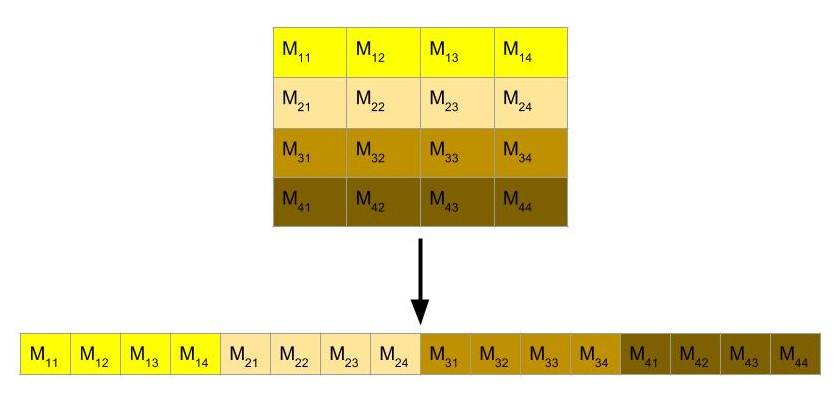
\includegraphics[width=\linewidth,height=12cm,keepaspectratio]{Figures/flatten}
		\caption[flattening 2d matrix]
		{flattening 2d matrix to row-wise 1d vector}
	\label{fig:33}	
	\end{figure}
			
	The embedding process could be easily generalized if c is vectorized to values - set, then the dimension of $\alpha$ would be:\\ 
	$\prod_{i=1}^{2n}c_i$ , which equivalent to the number of vertices in the “discretized” space of the problem.
	In order to finally receive a distance/similarity/dis-similarity function, we apply inner product between $\alpha$  vector and a learned weights vector (equivalent to the $W$ matrix from the $1D$ scenario).

	
	\begin{algorithm}
				\caption{Embedding Method for ID N-Dimensional Pairs dataset}
				\begin{algorithmic}
				 
				
				\REQUIRE $L$ sized, vectorized n-dimensional pairs dataset
				\REQUIRE set of centers per dimension - $C$
				\ENSURE $\overrightarrow{\phi}$: $L$ sized set, embedded, sparse vectors\\
				
				\STATE \textbf{Find centers vectors}
				\STATE V shall be a set of centers - vectors
				\FORALL{dim in $n$}  
				\STATE $V_{dim} \leftarrow centers \quad vector \quad per \quad dim$
				\ENDFOR
				
				\STATE \textbf{Find embedded coefficients for all dataset}
				\STATE $\overrightarrow{\phi} = C^{2n}$ length empty $\overrightarrow{\phi}$ embedded vectors
				\STATE concat all pairs into a single vector $\overrightarrow{p}$
				\FORALL{$\overrightarrow{p}$ in $L$}
				\STATE find $\overrightarrow{p}$ bounding hypercube 
				\STATE find $\overrightarrow{p}$ bounding simplex (permutation method)
				\STATE $\overrightarrow{\lambda} \leftarrow$ find $\overrightarrow{p}$ barycentric coefficients 
				\STATE $\overrightarrow{\hat{\lambda}} \leftarrow$ normalize($\overrightarrow{\lambda}$)
				\ENDFOR
				\STATE \textbf{Assign}
				\FORALL{$\overrightarrow{\phi}$ in $emb-set$}
				\STATE $inds \leftarrow$ find vertices from hypercube and simplex locations
				\FORALL{$i$ in $inds$}
				\STATE $\overrightarrow{\phi}_{(i)} \leftarrow \overrightarrow{\hat{\lambda}}(j(i))$ -- j is the assigning function between the coef. vector and embedding vector
				\ENDFOR
				\ENDFOR
				
				\RETURN $\overrightarrow{\phi}$
	
				
				\end{algorithmic}
			\end{algorithm}
	
\break	
\section{Non-euclidean non-embeddable Metrics example}

Let us display an example of a useful application to IDDND method.
As described in the introduction chapter{}, IDDND method overcomes two main issues:

\begin{enumerate}
	\item \textbf{distortion} issues cause when applying euclidean metrics on a given arbitrary dataset. 
	\item \textbf{Metrics} are not necessarily applied on dissimilarities problems
\end{enumerate}

We demonstrate a theoretical use case constrained by those 2 conditions, and see how our method would overcome those and fits a proper model to a non-embeddable dataset.
\\ \\ 
\newcommand{\centert}{2.66}

\begin{figure}[h]
	\centering

	\begin{tikzpicture}

	\draw (0,0) node[anchor=north]{$\overrightarrow{x_2}$}
	-- (8,0) node[anchor=north]{$\overrightarrow{x_3}$}
	-- (4,6.928) node[anchor=south]{$\overrightarrow{x_1}$}
	-- cycle;
	
	%\draw (4,\centert) node[anchor=north]{$\overrightarrow{x_0}$}
	\draw (0,0) -- (4,\centert);
	\draw (8,0) -- (4,\centert);
	\draw (4,6.928) -- (4,\centert);
	\node at (4.5,2.9) {$\overrightarrow{x_0}$};
	
	\node[green] at (1.8,3.7) {$2$};
	\node[green] at (6.2,3.7) {$2$};
	\node[green] at (4,-0.5) {$2$};
	
	\node[green] at (3.8,4.7) {$1$};
	\node[green] at (2.2,1.8) {$1$};
	\node[green] at (5.8,1.8) {$1$};
	
	\draw[black,fill=black] (0,0) circle (.5ex);
	\draw[black,fill=black] (8,0) circle (.5ex);
	\draw[black,fill=black] (4,6.928) circle (.5ex);
	\draw[black,fill=black] (4,\centert) circle (.5ex);
	
	\end{tikzpicture}
	
	\caption[triangle non-embeddable dataset]
	{non-embeddable dataset scheme, describing a 2D triangled set, where 4 centers represents 4 data groups which their average distances shown in \textcolor{green}{green}}
	
	\end{figure}
	
	This theoretical set form applies a non-euclidean embeddable metrics, which we now prove that a euclidean metrics is unable to embed it. \\ \\
	Based on euclidean metrics assumptions, assumed there is an integer $k$ , such that a function $f$ applies: \\
	
	$f \: : \: \{  \overrightarrow{x_1}, \overrightarrow{x_2} , \overrightarrow{x_3} , \overrightarrow{x_4}\} \rightarrow \Re^k$ \\
		
	Where $\overrightarrow{x_i}$ are samples from each one of data centers, and $f$ preserves the distances. \\
	
    As triangle-inequality is tight for: $\overrightarrow{x_4} , \overrightarrow{x_1} , \overrightarrow{x_2}$ ,\\
	
	and $f(\overrightarrow{x_4}) ,f(\overrightarrow{x_1}) ,f(\overrightarrow{x_2})$ are collinear in $\Re^k$ \\ 
	
	From set formation symmetry property, the same colinearity applies on:
		
	$f(\overrightarrow{x_3}) ,f(\overrightarrow{x_1}) ,f(\overrightarrow{x_2})$ \\ 
	
	This common colinearity of those tuples leads to the following equation:
	
	$\left \| f(\overrightarrow{x_4}) - f(\overrightarrow{x_3})  \right \|_2 == 0$ \\
	
	But this fact is contradicting that 
	
	$ d(\overrightarrow{x_4}\ , \overrightarrow{x_3}) = 2 $
	
	
	





	






\chapter{Interpolated Discretized Single objects Embedding} % Main chapter title

\label{Chapter4} % For referencing the chapter elsewhere, use \ref{Chapter1} 

Data objects may describe an abstracted format of any data type exists, such images, video, audio, text etc.
\textbf{Single} objects embedding may assist in classification and regression tasks, by emphasizing differences among data samples, without spending lots of time and memory.
\\
In this section we describe how we perform our ID method on such single vectors domain.



\section{Discretization}

We begin by dataset discretization, which is equivalent in all the use cases displayed in our method.
Dataset is being discretized by performing clustering on its dimensions and find C centers for discretization. This step should maintain the dataset extreme values within the extreme values of the C vector (so in the interpolation phase there will be valid values for all data elements \ref{fig:4.1}.


\begin{figure} 
\centering
		
		\begin{pmatrix} v_1 ,  v_2 , \dots , \dots , v_{n-1}, v_n} \end{pmatrix}\\
		
		\begin{pmatrix}
			m_{1,1}&   \dots&   \dots&   \dots& m_{1,n}\\
			\vdots& \ddots &        &        & \vdots \\
			\vdots&        & \ddots &        & \vdots  \\
			\vdots&        &        & \ddots & \vdots  \\
			m_{C-1,1} &        &        &        & m_{C-1,n}  \\
			m_{C,1}  & \dots  & \dots  & \dots  & m_{C,n}
		\end{pmatrix}
		\caption[discretization matrix]
		{discretization points set $W$ as built from a single dimensional dataset. this set is vectors' length may vary among dimensions}
\label{fig:4.1}		
\end{figure}


\section{Interpolation}

Interpolation of a given dataset, after extracting its discretization centers, is performed by the following sequence:

\begin{itemize}
\item Find bounding hypercube
\item Find bounding simplex
\item Find sample’s correlated coefficients per simplex vertices as described at \ref{hypercubes}
\item Convert coef. vector to  normalized format. $v_i \in [0,1]$  by dividing with the volume of the simplex
\end{itemize}

\section{Assigning}

Here we proceed embedding process by assigning the normalized coefficients vector to their indices in the embedded vector.
In the 1d scenario, the embedded vector would be sized as centers number per dimension - $C$, powered by dimension length - $n$



\begin{algorithm}
		\caption{Embedding Method for ID N-Dimensional single vectors dataset}
		\begin{algorithmic}
 
		
		\REQUIRE $L$ sized, vectorized n-dimensional dataset
		\REQUIRE set of centers per dimension - $C$
		\ENSURE $\overrightarrow{\phi}$: $L$ sized set, embedded, sparse vectors\\
		
		\STATE \textbf{Find centers vectors}
		\STATE V shall be a set of centers - vectors
		\FORALL{dim in $n$}  
		\STATE $V_{dim} \leftarrow centers \quad vector \quad per \quad dim$
		\ENDFOR
		
		\STATE \textbf{Find embedded coefficients for all dataset}
		\STATE $\overrightarrow{\phi} = C^{n}$ length empty $\overrightarrow{\phi}$ embedded vectors
		
		\FORALL{$\overrightarrow{p}$ in $L$}
		\STATE find $\overrightarrow{p}$ bounding hypercube 
		\STATE find $\overrightarrow{p}$ bounding simplex (permutation method)
		\STATE $\overrightarrow{\lambda} \leftarrow$ find $\overrightarrow{p}$ barycentric coefficients 
		\STATE $\overrightarrow{\hat{\lambda}} \leftarrow$ normalize($\overrightarrow{\lambda}$)
		\ENDFOR
		\STATE \textbf{Assign}
		\FORALL{$\overrightarrow{\phi}$ in $emb-set$}
		\STATE $inds \leftarrow$ find vertices from hypercube and simplex locations
		\FORALL{$i$ in $inds$}
		\STATE $\overrightarrow{\phi}_{(i)} \leftarrow \overrightarrow{\hat{\lambda}}(j(i))$ -- j is the assigning function between the coef. vector and embedding vector
		\ENDFOR
		\ENDFOR
		
		\RETURN $\overrightarrow{\phi}$

		
		\end{algorithmic}
	\end{algorithm} 
% Chapter 1

\chapter{Time Complexity} % Main chapter title

\label{Chapter5} % For referencing the chapter elsewhere, use \ref{Chapter1} 

%----------------------------------------------------------------------------------------

% Define some commands to keep the formatting separated from the content 
%\newcommand{\keyword}[1]{\textbf{#1}}
%\newcommand{\tabhead}[1]{\textbf{#1}}
%\newcommand{\code}[1]{\texttt{#1}}
%\newcommand{\file}[1]{\texttt{\bfseries#1}}
%\newcommand{\option}[1]{\texttt{\itshape#1}}

%----------------------------------------------------------------------------------------
Time complexity for each step of the IDDND function building is displayed in this section. 
Learning / training timing was excluded and will be discussed at ()


\section{Discretization}

	Discretization implementation is not specified in this paper since we are using a OTS method such $k-means$ clustering algorithm, although This step may be applied by various methods. 
	The common ones are k-means or their variation. We will try to refer to $k-means$ \ref{---} based methods.
	Though the problem of finding the global optimum of the $k-means$ objective function:
	
	\begin{equation}
	arg\min_s\sum_{i=1}^{k} \sum_{x_j \in S_i}^{}\|x_j - \mu_i \|^2
	\end{equation}
	
	is NP-hard[].
	
	However, running a fixed number i of iterations of the standard algorithm consumes only: \\ \\ \\
	\textbf{$O(i \dot k \dot n \dot d)$} \\ \\
	Where:
	i - convergence iterations \\
	k - number of means \\
	N - dataset samples \\
	n - object dimension \\
    
    for n points in d dimensions
	






\section{Interpolation}

As described above(), we divide the interpolation phase time complexity for several phases:




\section{Find the bounding hypercube}

Finding a given vector’s bounding box is actually finding a bounding pair for each element in this vector. Since the means vectors are sorted then this step takes n times (for n dimensions) $log(n)$ , which is the time complexity for binary search.
In total, time complexity of this step:  

\\
\textbf{$O(nlog(n))$}
\\


\section{Find the bounding simplex}


Finding the bounding simplex is equivalent to find an obeying permutation over the given vector.
Time complexity for this step is therefore: \\$O(nlog(n))$\\. While using common sorting algorithms such Quicksort[]/Merge Sort[]/Timsort[].








\section{ID coefficients extraction}

In the step, we take in matter only the second attitude shown above since it is faster.
Computing the coefficients is also possible in $O(n)$.
We can compute the first index in $O(n)$ and do additional $O(n)$ updates each with a time complexity of $O(1)$ for computing the other indices, so in total this step take only $O(n)$.

total time complexity for the interpolation step method is: \\

$ O(nlog(n)) + O(nlog(n)) + O(n) = O(nlog(n)) $





\section{Assigning}

The embedding of the sparsed vector is purely flattening a matrix into a vector shape, which takes $O(1)$



% Chapter 1

\chapter{Memory Complexity} % Main chapter title

\label{Chapter6} % For referencing the chapter elsewhere, use \ref{Chapter1} 

%----------------------------------------------------------------------------------------

% Define some commands to keep the formatting separated from the content 
%\newcommand{\keyword}[1]{\textbf{#1}}
%\newcommand{\tabhead}[1]{\textbf{#1}}
%\newcommand{\code}[1]{\texttt{#1}}
%\newcommand{\file}[1]{\texttt{\bfseries#1}}
%\newcommand{\option}[1]{\texttt{\itshape#1}}

%----------------------------------------------------------------------------------------


In this section we provide a method for applying dimensional reduction of the multidimensional scenario, by grouping significant small subsets of the data and concatenating them after embedding. 


\section{Definition}

We define a generalized ID function by:

\begin{equation}
ID_(\overrightarrow{x_1} , \overrightarrow{x_2} ; S) = [ ID(\overrightarrow{x_1}_[S_1],\overrightarrow{x_2}_[S_1]) , \dots , \dots , ID(\overrightarrow{x_1}_[S_g],\overrightarrow{x_2}_[S_g])  ]
\end{equation}

where $S$ is the defined sub-domain group: \\ 

$\{S_i\}_{i=1}^g \qquad,\qquad S_i\subseteq [1, \dots , n] \qquad , \qquad g \in [1, \dots , n]$ \\ 

Where $g$ represents a sub domain which extracts valid demandable information to the user. \\ \\ \\


For example when applying ID embedding on \textbf{SIFT[]} descriptors, a certain user may involve only neighbor pairs, where another one may involve just bin-to-bin pairs.

\subsection{SIFT Example}

when applying ID on SIFT [] descriptors (for template matching),  n is 128, which causes time and memory complexity to be scaled by 1282=16384. 
If one user desires, and physically ables to reduce this coefficient, we developed the following generalization.

\begin{figure} \label{s1}
	    \centering
		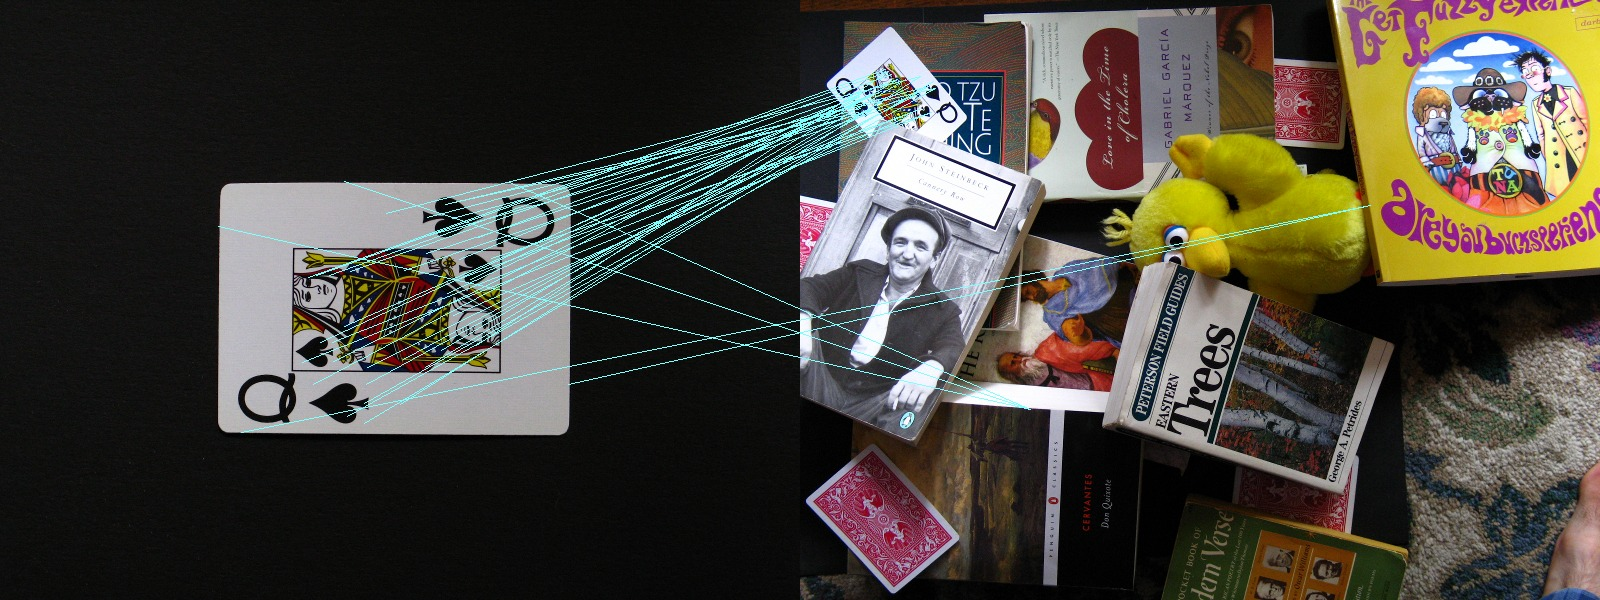
\includegraphics[width=\linewidth,height=12cm,keepaspectratio]{Figures/sift1}
		\caption[flattening 2d matrix]
		{flattening 2d matrix to row-wise 1d vector}
	
\end{figure}
	
	
	
\begin{figure} \label{s2}
		\centering
	
		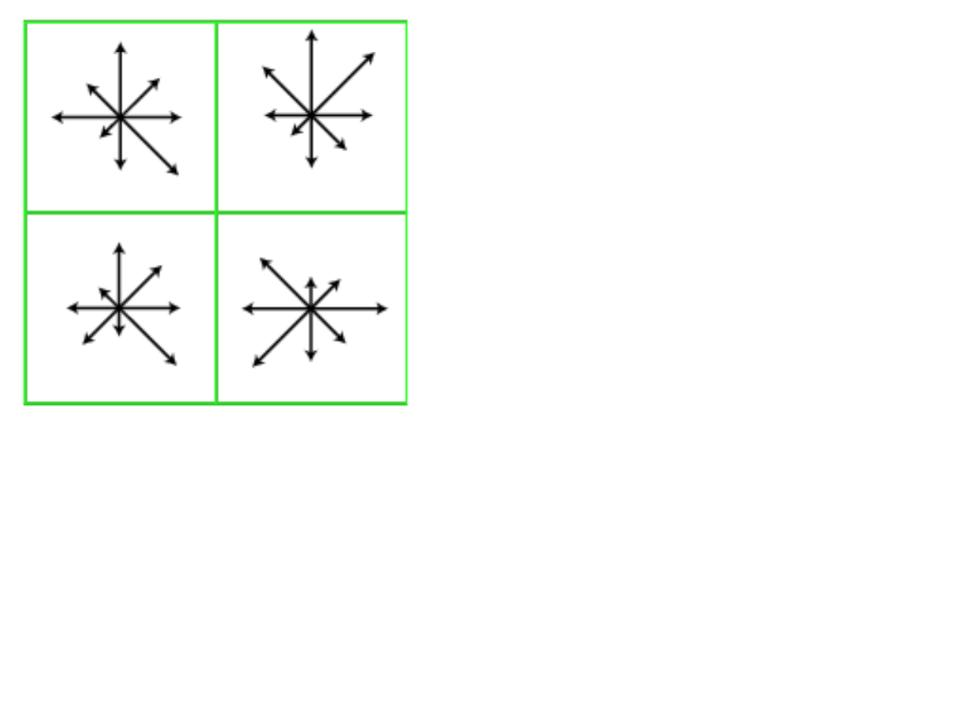
\includegraphics[width=12cm,height=12cm,keepaspectratio]{Figures/sift2}
		\caption[flattening 2d matrix]
		{flattening 2d matrix to row-wise 1d vector}
	
\end{figure}

 
% Chapter 1

\chapter{Learning} % Main chapter title

\label{Chapter7} % For referencing the chapter elsewhere, use 


In this section described the learning phase of the $IDDND$ method.\\
Learning a single vectors dataset will be described further, since it is the simpler scenario.
In general, since our method is embedding objects or object pairs to sparse vectors set, we can use this quality in order to accelerate learning phase of the process.


\section{Learning the Classification Function}

As described above (), our current method is handling similarity detection between two n-dimensional vectors. This can of course be generalized to any classification/clustering matter.

Let X be a set of raw data vectors. Each vector in this set may represent a single object, for any type of classification analysis. 

In this scenario we obtain object pairs similarity problem.
Let us assign an indexing system for this labeled pairs dataset as follows:

\begin{equation}
P = \begin{bmatrix}
p_{11} & p_{12}\\ 
 \vdots & \vdots \\ 
p_{i1} & p_{i2}\\ 
 \vdots & \vdots \\ 
p_{k1} & p_{k2}\\ 
\end{bmatrix}
\overrightarrow{y} = \begin{bmatrix}
y_{1} \\ 
 \vdots  \\ 
y_{i} \\ 
 \vdots  \\ 
y_{k} \\ 
\end{bmatrix}
\end{equation}

Where $P$ set refers to $X$ set indices and tghsgfds refers to the vectors label as follows:
\definecolor{darkgreen}{RGB}{0, 140, 0}
\begin{equation}
y_{i} = \left\{
\begin{array}{ll}
     
      {\textcolor{darkgreen}{ -1 \: \: if \:  \overrightarrow{x_{pi1}}\: and \: \overrightarrow{x_{pi2}} \:are\: similar} \\
      {\textcolor{red}{ +1 \: \: if \:  \overrightarrow{x_{pi1}}\:  and \: \overrightarrow{x_{pi2}} \:are\: non-similar} \\

\end{array} 
\right.
\end{equation}

We define a classification (similarity) function:


\begin{equation}
similar(\overrightarrow{x_{1}} , \overrightarrow{x_{2}})= \left\{
\begin{array}{ll}

{\color{darkgreen}{ -1 \: \: if \:  d(\overrightarrow{x_{1}} , \overrightarrow{x_{2}})\,=\,IDD(\overrightarrow{x_{1}} , \overrightarrow{x_{2}})\cdot \overrightarrow{w} < t  } \\
{\color{red}{ +1 \: \: otherwise} \\

\end{array} 
\right.
\end{equation}

Where A pair of vectors is similar if and only if their ID distance result is smaller than a threshold parameter (t).
This function is identical to a classification function of a standard binary SVM classification method [80], which looks like the following:

Where 
t - threshold which learned by an optimization process
- weight vector of the problem which is also learned by an optimization process.

We now address describing the optimization of the learning step for achieving optimal model for a certain data set.



\section{Efficient Stochastic Gradient Descent}

Stochastic Gradient Descent (SGD) is a stochastic approximation of the gradient descent optimization method for minimizing an objective function that is written as a sum of differentiable functions.

SGD is a simple yet very efficient approach to discriminative learning of linear classifiers under convex loss functions such as our learning function.

As Shalev-Shwartz et al. POLA [67], we can learn our weights (including t parameter):

\begin{equation}

\overrightarrow{w}^{opt} , t^{opt} =\\ 
\underset{\overrightarrow{w} , t}{argmin} 


(\frac{1}{2}\left \| 

\overrightarrow{w} - \overrightarrow{w}^{reg} \right \|_2^2 + \\ C \sum_{i=1}^{k}max(1-(IDD(\overrightarrow{x_{p_i1}} , \overrightarrow{x_{p_i1}}) \cdot \overrightarrow{w} - t)y_i , 0))



\end{equation}
% Chapter 1

\chapter{Experiments} % Main chapter title

\label{Chapter8}

In this chapter we display a novel usage to our new the $ID$ method attributes and qualities. Here we will use our $ID$ method in order to obtain a \textbf{perceptual colors distance metric learning} \cite{perp_color}, which is a high demanded function in computer vision region.\\ 
Our examination is based and referring to \cite{perp_color} and \cite{c2lm} papers, which developed a local metric embedding method for this problem. 

This set of experiments models a perceptual color difference metrics, based on various color samples originated from several cameras, angles, illuminations etc.
\\

Our $ID$ method would be examined in this section solely by the original experiment's accuracy measures - Mean Absolute Error \cite{MAE}, along various parameters such number of centers per dimension, and different datasets assembly.
\\
Further discussion will refer to the various exams may apply on our $ID$ method according to our described theory.

\section{Experiment Procedure}

\textbf{object pairs ID embedding} \ref{Chapter3} will be demonstrated by applying its embedding method over pairs which was taken and labeled from the Farnsworth-Munsell 100 hue-test set \cite{farnsworth}.
\subsection{Dataset}

Dataset of this experiment is assembled from single color patches, which displayed in a set of images, where each image was generated by a specific set of image features, such illumination, camera type (4 different cameras are involved in the dataset creation) , lance type , background etc.

\begin{figure}[H] \label{set_ds}
			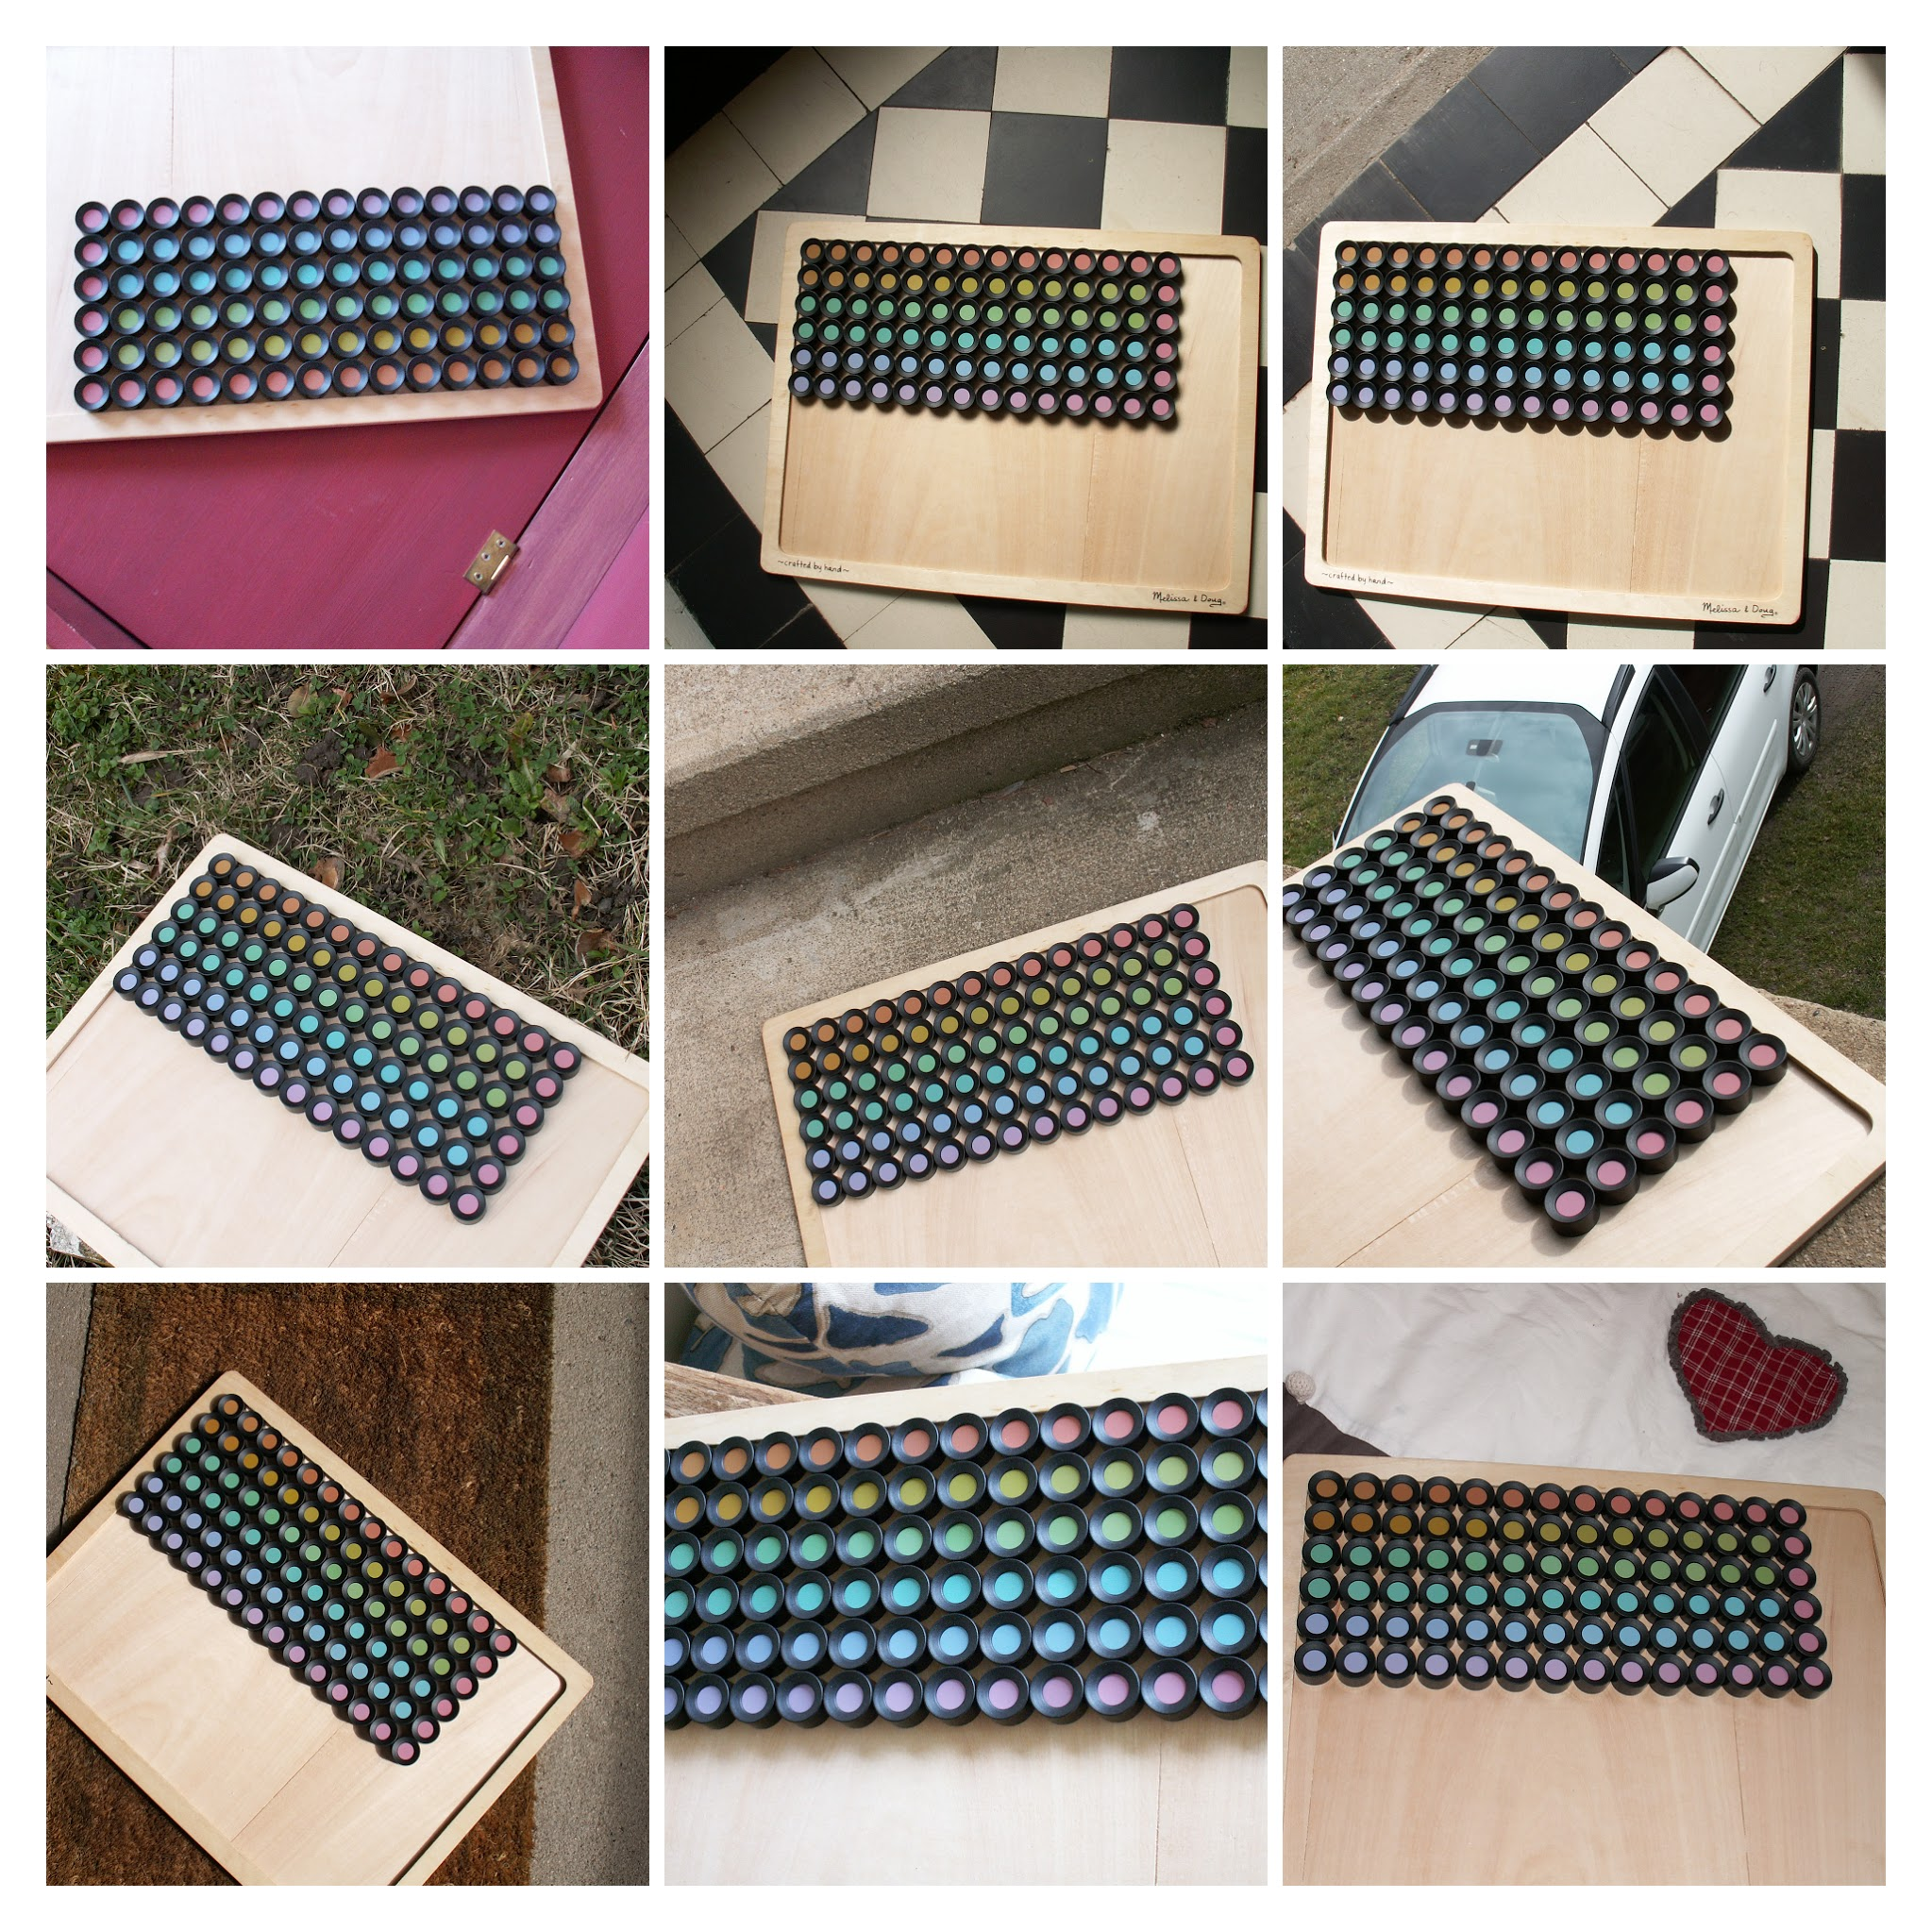
\includegraphics[width=\linewidth,height=12cm,keepaspectratio]{Figures/set_ds}
			\caption[set ds]
			{dataset patches original images formats}
\end{figure}

For each color patch, a $L^*A^*B^*$ \cite{lab} coordinates are given. 
Since the pairs of patches should be close by their CIELAB \cite{CIELAB} coordinates in order to adapt a good color difference assessment, a set in the final dataset is only a set of patches, where its CIELAB euclidean distance is relatively close, i.e. $\Delta E \leq 5$ .


%\begin{figure}[H] \label{patch_positions}
%			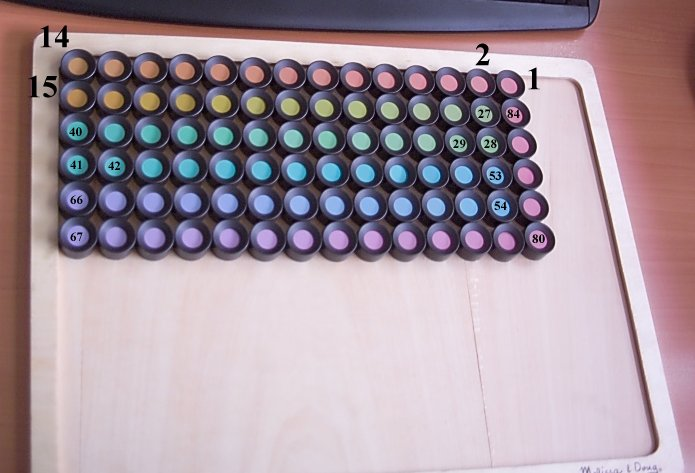
\includegraphics[width=\linewidth,height=12cm,keepaspectratio]{Figures/patch_positions}
%			\caption[color patches order in every samples image]
%			{patches order}
%\end{figure}


\subsection{Models to train}
\label{color_cam}
Then, $ID$ learning method will try to learn some similarity models according to a couple of test conditions:

\begin{itemize}
	\item \textbf{unseen colors} - dividing the entire patches set into train-test sets
	\item \textbf{unseen cameras} - assigning 3 out of 4 cameras sets as train set, and make the remained camera set as test set. \\
		training set cameras:
		\begin{itemize}
			\item Kodak DCS	Pro 14n
			\item Konica Minolta Dimage Z3
			\item Nikon Coolpix S6150
		\end{itemize}	
		
		test set camera:	
		\begin{itemize}
			\item Sony DCR-SR32
		\end{itemize}
		
\end{itemize}

\subsection{Interpolation}
Data dimension in our scenarios is of course $n=3$ (for lab/RGB \cite{RGB} coordinates), and for an object pair the dimension is $2n=6$. \\
As described in \ref{Chapter3}, interpolation is performed dimension-wise along the training set, after selecting data center per dimension by manual or automatic (k-means) method.
\\
In our experiment we have selected cross validation \cite{cross_val} over certain fold number of our dataset for assessing the optimal number of centers per dimension, and find those by using k-means \cite{kmeans} algorithm.





For the selected number of extracted centers we add two extreme points for applying proper interpolation for data values beyond limits of the discovered centers.
\\
Now that we have found data centers for each dimension we apply our interpolation method \ref{Chapter3} on our data (on both train-test sets) and extract a $\overrightarrow{a} \in \Re^3$ coefficient vector per color patches pair, which is ready to be embedded.


\subsection{Embedding}
Our dataset is now embedded by applying an embedding of the coefficient vectors on a sparse form such: 
\vskip5pt
$\overrightarrow{e} \in \Re^{2\prod_{i=1}^{n}{length(\overrightarrow{c_i})}}$ 
\vskip5pt
where $n = 3$.
\vskip5pt
Each coefficient vector element is assigned to the exact simplex index in the $\overrightarrow{e}$ embedded vector.
\\

\subsection{Learning}
Learning phase is performed on a linear regression model training process.
As described on \ref{learn_regression}, we learn by using \textbf{Stochastic Gradient Descent} \cite{SGD} optimization algorithm, regularized by a known distance such $\lone$. \\
Loss function of the training process would be a generalized Mean Average Error \cite{MAE} loss function, constrained by our semi-metrics critireas for model divergence as described in the learning chapter \ref{Chapter5}:
%\begin{equation}
%\wopt & = \\
%& \argmin_{\wadd} 
%\Bigg( 
%\learningregtwo + 
%\\
%& C \sum_{i=1}^{\pairsnum}
%\Big(
%\distreg(\xvpairsindexifirst,\xvpairsindexisecond) + 
%\ope(\xvpairsindexifirst,\xvpairsindexisecond) \cdot \wadd - \\
%& \simlabel_i\Big)^2
%\Bigg)
%\end{equation}


\subsection{Assessment}
Models assessment is applied by following criteria:
\begin{itemize}
\item \textbf{MAE} - Mean Absolute Error
\end{itemize}

The test set of each experiment is processed by our embedding method and a  distance figure is calculated. This figure $y_i^{test}$ is being compared to the predicted label for each sample by assembling the MAE index:
\begin{equation}
MAE = \frac{1}{n} \cdot \sum_{i = 1}^{n}{|y^{pred}_i - y^{test}_i|}
\end{equation}
Where n is test set size. \\


\section{Results}

Let us describe our results being compared to the original paper results as described in \ref{original paper results}.
We display the experiments for each data splitting (camera/color). 
Our experiments performed by applying cross validation algorithm mentioned at  \ref{cross_validation}.
Let us observe the experiments performed on data splits described \ref{color_cam}.
\\

Along all the experiments we perform sweep over the number of centers per dimension $c \in [2,10]$, which will describe the behavior of all models over datasets' dispersion.
\\
We display several examinations of our results:
\begin{itemize}
	\item \textbf{regularizers scan} - $L1, L2, \Delta E$
	\item \textbf{train .vs. test} sets error
	\item \textbf{unseen colors .vs. unseen cameras}	
\end{itemize}
We also describe a comparison of results based centers extracted by cross validation algo.


\subsection{Cross-Validation Centers}

\begin{itemize}
	\item Unseen Colors

Unseen color case was assembled by a certain percentage of all data set as train set, and the rest as test set. In this experiment we have taken the train set size to be $80 \%$ of the total data set.

	\subsubsection{Dataset properties}
	
	From a total 13500 patches pairs set, the divided train-test sets amounts are:
	\begin{table}[H]
		\centering
		\label{test_train1}
		\begin{tabular}{|c|c|}
			\textbf{set} & \textbf{size} \\ \hline \textbf{train} & \textbf{10800} \\ \hline
			\textbf{test} & \textbf{2700} \\ \hline
		\end{tabular}
		\caption{train/set ratio = $4/1$}
	\end{table}
		
	\subsubsection{Centers locations}
	
	Centers locations are shown as extracted via cross-validation \ref{cross_validation} for finding optimal number of centers per dimension, and k-means for extracting centers values. \\
	k-means actually found only the inner centers, since the outer centers are fixed bounds.\\
	
	
	\begin{matrix}  \qquad  c_0 \quad  \qquad c_1 \quad  \qquad c_2 \end{matrix}\\
			
	
	\begin{pmatrix}
\label{key}     0.0 &     0.0 &    0.0\\
				44.5 &   30.35 &    43.13 \\
				84.4 &   80.28 &    83.43 \\
				161.59 &   150.96 &   168.81\\
     		 255.0 &  255.0 &   255.0 \\
	\end{pmatrix}
	
	\vskip10pt


	\subsubsection{Experiment Figures}
	
	Our model provides the following figures:

	\begin{itemize}
	\item 	p-value = $3.9 \cdot 10 ^{-03}$
	\item 	MAE = $0.80$
	
	\end{itemize}


\item Unseen Camera
%\subsection{Unseen Camera}

Unseen camera scenario was assembled by assigning one of the cameras involved in dataset generation as test set, where the other 3 functions as train set.


	\subsubsection{Dataset properties}
	
		From a total 13500 patches pairs set, the divided train-test sets amounts are:
		\begin{itemize}
			\item \textbf{train set size} = $8084$ 
			\item \textbf{test set size} = $5416$ (Sony DCR-SR32 camera set)
		\end{itemize}
		
		\begin{table}[H]
			\centering
			\label{test_train2}
			\begin{tabular}{|c|c|c|}
				\hline
				\textbf{set} & \textbf{size} & \textbf{cameras} \\ \hline \textbf{train} & \textbf{8084} & \textbf{Kodak DCS Pro 14n, Konica Minolta Dimage Z3,
					Nikon Coolpix S6150} \\ \hline
				\textbf{test} & \textbf{5416} & \textbf{Sony DCR-SR32}\\ \hline
			\end{tabular}
			\caption{train/set ratio = $3/2$}
		\end{table}
		

	\subsubsection{Centers locations}
	
	Centers locations are shown as extracted via cross-validation \cite{cross_val}. for finding optimal number of centers per dimension, and k-means for extracting centers values.\\
	k-means actually found only the inner centers, since the outer centers are fixed bounds.

	\vskip30pt
	\begin{matrix}  \qquad  c_0 \quad  \qquad c_1 \quad  \qquad c_2 \end{matrix}
			
	
		\begin{pmatrix}
		0.0 &     0.0 &    0.0\\
		50.6 &   90.55 &    84.43 \\
		101.54 &    &   \\		
		171.29 &   160.98 &   158.21\\
		255.0 &  255.0 &   255.0 \\
	\end{pmatrix}
	\\

	As seen in centers list, edges are equal per dimension $[0.0 , 255.0]$ for data bounding.
	
	\subsubsection{Experiment Figures}	
	Our model provides the following figures:	
	\begin{itemize}
	\item 	p-value = $4.5 \cdot 10 ^{-05}$
	\item 	MAE = $0.79$
	
	\end{itemize}

\end{itemize}


\subsection{Regularizers Comparison}



\subsection{Train/Test sets Comparison}


\subsection{Unseen colors/Unseen camera sets Comparison}





\section{Comparison}

\begin{figure}[H] 
	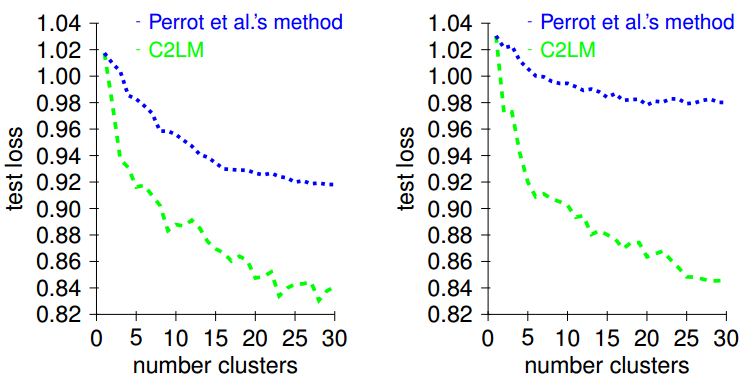
\includegraphics[width=\linewidth,height=10cm,keepaspectratio]{Figures/orig_paper_charts}
	\caption[orig res]
	{original paper test loss charts, as function of cluster numbers}
	\label{original paper results}			
\end{figure}


Let us treat our results versus the original paper's results.\\

While \cite{perp_color} (regression) method
\ref{original paper results} shows results for either camera/color scenarios for model assessment with MAE. \\
The \ref{original paper results} charts' x - axes describes the number of clusters been used in their embedding algorithm. \\
Their minimal values on both scenarios are \textbf{ > 0.82 for MAE}, where our results are \textbf{ < 0.80 for MAE}, all for a $p-value$ with a similar magnitude to theirs. \\
As clearly seen, our results applies the following conditions:
\begin{itemize}
	\item Slight outperforming reference original paper error scores
	\item Small p-values which proves the validity of our method, since there is a reasonable assumption that our models provide close dataset approximation
	\item Overfitting avoidance by applying cross validated centers based on our training set solely.
\end{itemize}

This information is a meaningful confirmation of the assumption that our method is valid to work with in terms of reliability. In the following chapter we will discuss the further explorations should be performed to examine the rest of performance criterias mentioned above.
 
% Chapter 1

\chapter{Conclusions and discussion} % Main chapter title

\label{Chapter9} 

\section{Summary}

In this work we have proposed a new embedding method for a single vector and for a pair
of vectors. This embedding method enables: 
\begin{enumerate}
	\item efficient classification and regression of functions of single vectors
	\item efficient approximation of distance functions
	\item general, non-Euclidean, semimetric learning
\end{enumerate}.
For the best of our knowledge, this is the first work that enables learning any general, non-Euclidean, semimetrics.\\ 
That is, our method is a universal semimetric learning and approximation method that can approximate any distance function with as high accuracy as needed with or without semimetric constraints.\\
In this work, we have displayed a detailed exploration of our $ID$ method, describing its basic classification/regression algorithmic flow for objects embedding and its applications options.\\

We have described how it may be applied on pair objects matters, such similarity/dissimilarity problems \ref{Chapter3}.\\

Also described how to apply our method on single objects embedding problems, for cases such classification/regression problems \ref{Chapter4}.\\

On chapter \ref{Chapter5}, the learning phase of the embedding method was described, detailing a specific adaptation to SGD \cite{SGD} algorithm in order to fit our data types to optimize the optimization process of loss convergence.\\

Chapter \ref{Chapter6} handles the time complexity issues related to the embedded objects. Each step in the process is analyzed in terms of current complexity analysis of the general method.\\

Chapter \ref{Chapter7} handles the memory issues related to the embedded objects, which are originally sparsed, and how it may be treated in order to save memory.\\

Chapter \ref{Chapter8} examines our $IDD$ method on e test case displayed by \cite{perp_color}, which studies method to observe perceptual colors difference. Here we have validated the correctness of our method by displaying out-scoring results in comparison to original articles results.

\break
\section{further exploration}

This work displays a continuous non-linear embedding method for any desired classification/regression task. In chapter \ref{Chapter8} we displayed an accuracy exploration of our method, on the object pairs embedding scenario. \vskip10pt
In addition to this examination, the following objectives may be observed:

\begin{itemize}
	\item \textbf{various centers per dimension} may be a good valuation of the optimal condition per problem, in case cross validation may treat single dimension at a time. By optimizing several dimensions in one shot, one can decide of a fixed number of centers for all dimensions, which may be still optimized in matters of accuracy, time and memory.
	\item \textbf{Memory} consumption may be observed among various embedding method include ours, while using our memory saving tips at chapter \ref{Chapter6}, where in our method (and in \cite{perp_color}, number of centers/clusters is a valid argument to parameterize in this kind of comparison)
	\item \textbf{time} complexity may also taken in comparison among various object-embedding methods, while using our chapter \ref{Chapter7} theories.
	\item \textbf{end-to-end application embedding} such image segmentation as shown in \cite{perp_color}, may assist evaluating this method
	\item \textbf{single objects embedding} may also be inspected for some classification/regression task, again with all parameters mentioned above (accuracy, time, memory)
\end{itemize}

 

%----------------------------------------------------------------------------------------
%	THESIS CONTENT - APPENDICES
%----------------------------------------------------------------------------------------

\appendix % Cue to tell LaTeX that the following "chapters" are Appendices

% Include the appendices of the thesis as separate files from the Appendices folder
% Uncomment the lines as you write the Appendices

% Appendix A

\chapter{Appendix Title Here} % Main appendix title

\label{AppendixA} % For referencing this appendix elsewhere, use \ref{AppendixA}

Write your Appendix content here.
%\include{Appendices/AppendixB}
%\include{Appendices/AppendixC}
\section*{References}
As first example citation here is \cite{cover_trees}. 
Here is another example citation \cite{sift_lowe}



\printbibliography
%-------------------------------------------------------------------------------

\end{document}  

